\documentclass[aspectratio=169,10pt,fontset=none]{ctexbeamer}
\usepackage{fontspec}
\setCJKmainfont[AutoFakeBold=2]{Droid Sans Fallback}
\setCJKsansfont[AutoFakeBold=2]{Droid Sans Fallback}
\setCJKmonofont{Droid Sans Fallback}
\setsansfont{TeX Gyre Heros}
\usepackage{amsmath,amssymb,booktabs,tabularx,graphicx,tikz}
\usetikzlibrary{arrows.meta,positioning,calc,decorations.pathmorphing,fit}
\definecolor{Navy}{HTML}{17344D}
\definecolor{Teal}{HTML}{177E89}
\definecolor{Orange}{HTML}{C46536}
\definecolor{Muted}{HTML}{5D6D78}
\definecolor{Pale}{HTML}{EDF4F7}
\setbeamercolor{normal text}{fg=Navy,bg=white}
\setbeamercolor{structure}{fg=Teal}
\setbeamercolor{frametitle}{fg=Navy,bg=white}
\setbeamercolor{framesubtitle}{fg=Teal}
\setbeamercolor{block title}{fg=white,bg=Navy}
\setbeamercolor{block body}{fg=Navy,bg=Pale}
\setbeamercolor{alerted text}{fg=Orange}
\setbeamertemplate{navigation symbols}{}
\setbeamertemplate{itemize items}[circle]
\setbeamertemplate{bibliography item}[text]
\setbeamerfont{frametitle}{size=\large,series=\bfseries}
\setbeamerfont{framesubtitle}{size=\small}
\setbeamersize{text margin left=7mm,text margin right=7mm}
\setlength{\parskip}{1.5mm}
\setlength{\tabcolsep}{4pt}
\renewcommand{\arraystretch}{1.18}
\setbeamertemplate{footline}{%
  \hspace{7mm}\color{Muted}\fontsize{6.5}{8}\selectfont
  0918 calibration study\quad|\quad\insertsection
  \hfill\insertframenumber\,/\,\inserttotalframenumber\hspace{7mm}\vspace{2mm}}
\newcommand{\src}[1]{\vfill{\fontsize{7}{8.5}\selectfont\color{Muted}依据：#1\par}}
\newcommand{\ket}[1]{\lvert #1\rangle}
\newcommand{\takeaway}[1]{\begin{beamercolorbox}[sep=2mm,wd=\linewidth]{block body}\textbf{#1}\end{beamercolorbox}}
\tikzset{box/.style={draw=Navy,rounded corners=2pt,fill=Pale,align=center,minimum height=9mm,font=\small},
  flow/.style={-{Latex[length=2mm]},line width=.8pt,draw=Navy},
  drive/.style={draw=Orange,very thick},probe/.style={draw=Teal,very thick}}
\title{从 superconducting hardware\texorpdfstring{\\}{ }到 calibration 数据判断}
\subtitle{0918：实验流程、参考数据与需要检查的案例}
\author{Calibration study notes}
\date{2026 年 10 月 10 日}

\begin{document}
\begin{frame}[plain]
  \vspace{6mm}
  {\color{Teal}\small SUPERCONDUCTING QUBITS / CALIBRATION}\par
  \vspace{4mm}
  {\color{Navy}\LARGE\bfseries 从 superconducting hardware\\到 calibration 数据判断}\par
  \vspace{4mm}
  {\large 0918：实验流程、参考数据与需要检查的案例}\par
  \vspace{6mm}
  \begin{tikzpicture}
    \node[box,minimum width=3.4cm] (a) {Hardware\\电路实现什么功能？};
    \node[box,minimum width=3.4cm,right=7mm of a] (b) {Calibration\\如何控制和测量？};
    \node[box,minimum width=3.4cm,right=7mm of b] (c) {Data evidence\\数值在何时可信？};
    \draw[flow] (a)--(b);\draw[flow] (b)--(c);
  \end{tikzpicture}\par
  \vfill
  {\small 面向具有 Quantum Information / Computer Science 基础的听众}\par
  {\color{Muted}\footnotesize 2026-10-10\quad|\quad 正文：代表案例；附录：全部 47 个 review cases}
\end{frame}

\section{Hardware 与信号}
\begin{frame}{从 gate 到实验数据：中间有四个不同对象}
  \begin{columns}[T]
  \column{.48\linewidth}
  \begin{block}{Quantum operation}
    $X_\pi:\ket0\mapsto\ket1$，需要实际 pulse 实现。\\
    Measurement 的输出需要由电路 response 推断。
  \end{block}
  \begin{enumerate}
    \item \textbf{Device}：Transmon、resonator、coupler。
    \item \textbf{State}：$\ket0,\ket1$ 与 superposition。
    \item \textbf{Signal}：drive、probe、flux control。
    \item \textbf{Record}：数字化 response 或 assigned population。
  \end{enumerate}
  \column{.48\linewidth}
  \begin{block}{本报告要回答的问题}
    一个 calibration number 是怎样从\par
    \textbf{hardware + pulse sequence + measured response}\par
    中得到的？什么证据限制了它的解释？
  \end{block}
  \small
  0918 是六类 measurement 的集合，不是一个存储 qubit wavefunction 的 tensor。\par
  图中的 signal amplitude、pulse amplitude 和 population 是不同量。
  \end{columns}
  \src{Krantz et al. \cite{krantz}；0918 numeric records 与现有 calibration notes。}
\end{frame}

\begin{frame}{Transmon：用 nonlinear circuit 选择两个 energy levels}
  \begin{columns}[c]
  \column{.43\linewidth}
  \centering
  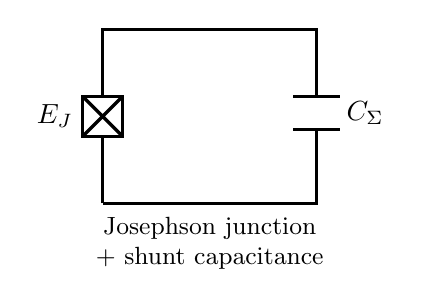
\begin{tikzpicture}[scale=.85]
    \draw[very thick] (0,0)--(0,2.6)--(3.2,2.6)--(3.2,1.6);
    \draw[very thick] (3.2,1.1)--(3.2,0)--(0,0);
    \draw[very thick] (2.85,1.6)--(3.55,1.6) (2.85,1.1)--(3.55,1.1);
    \draw[very thick,white,line width=4pt] (0,1.0)--(0,1.6);
    \draw[very thick] (-.3,1.0) rectangle (.3,1.6);
    \draw[very thick] (-.3,1.0)--(.3,1.6) (-.3,1.6)--(.3,1.0);
    \node[left] at (-.3,1.3) {$E_J$};\node[right] at (3.5,1.35) {$C_\Sigma$};
    \node[align=center,font=\small] at (1.6,-.6) {Josephson junction\\+ shunt capacitance};
  \end{tikzpicture}
  \column{.54\linewidth}
  \begin{tikzpicture}[x=1cm,y=.72cm]
    \draw[flow] (0,0)--(0,4.2) node[above,font=\small] {Energy};
    \foreach \y/\label in {.4/0,1.9/1,3.15/2}{
      \draw[very thick,Teal] (.5,\y)--(3.6,\y);
      \node[right] at (3.6,\y) {$\ket{\label}$};}
    \draw[<->,Orange,thick] (1.0,.4)--(1.0,1.9) node[midway,right] {$hf_{10}$};
    \draw[<->,Orange,thick] (2.8,1.9)--(2.8,3.15) node[midway,left] {$hf_{21}$};
    \node[font=\small] at (2,3.8) {$f_{10}\ne f_{21}$：anharmonicity};
  \end{tikzpicture}
  \end{columns}
  \vspace{2mm}
  \[
    H_q=4E_C\hat n^2-E_J\cos\hat\varphi,\qquad E_1-E_0=hf_{10}.
  \]
  \small $E_C=e^2/(2C_\Sigma)$；$E_J$ 为 Josephson energy；$\hat n$ 为 Cooper-pair number operator，$\hat\varphi$ 为 junction phase operator。这里省略 offset charge。\par
  \small 通常选择最低两个 energy eigenstates；higher levels 仍存在，误占据它们称为 leakage。$h$ 为 Planck constant。
  \src{自绘概念示意，非按比例；Krantz arXiv v5，Fig. 1、Eq. (16)，pp. 4--5 \cite{krantz}。}
\end{frame}

\begin{frame}{主流 chip：Qubit、readout resonator 与连接线路}
  \centering
  \begin{tikzpicture}[node distance=8mm,scale=.96,transform shape]
    \draw[probe] (0,3.4)--(12.8,3.4);
    \node[above,Teal] at (6.4,3.4) {Shared readout feedline：多个 probe frequencies 可共享一条线};
    \foreach \x/\name in {2.5/A,9.4/B}{
      \node[box,draw=Teal,minimum width=3cm] (r\name) at (\x,2.3) {Readout resonator \name};
      \node[box,minimum width=2cm] (q\name) at (\x,.65) {Transmon \name};
      \draw[probe] (\x,3.4)--(r\name.north);
      \draw[thick,dashed] (r\name.south)--(q\name.north) node[midway,right,font=\scriptsize] {coupling};
    }
    \draw[drive,-{Latex}] (.3,.65)--(qA.west);
    \node[font=\scriptsize,Orange,above] at (.85,.65) {Drive};
    \draw[drive,-{Latex}] (12.1,.65)--(qB.east);
    \node[font=\scriptsize,Orange,above] at (11.5,.65) {Drive};
    \node[box,minimum width=2.3cm] (coupler) at (6,.65) {Optional coupler};
    \draw[thick] (qA.east)--(coupler.west) (coupler.east)--(qB.west);
    \draw[flow] (6,-.55)--(coupler.south);
    \node[below,font=\small] at (6,-.55) {Flux control：可调 coupling / qubit frequency};
  \end{tikzpicture}
  \vspace{3mm}
  \begin{columns}[T]
    \column{.48\linewidth}\small
    \textbf{Readout resonator} 将 qubit state 编码到 microwave response。\par
    \textbf{Coupler / bus resonator} 用于 qubit 间 interaction；作用不同。
    \column{.48\linewidth}\small
    Chip 位于 dilution refrigerator，典型温度约 10--20 mK。\par
    Fixed-frequency 与 tunable Transmon 的线路配置可以不同。
  \end{columns}
  \src{通用 architecture 自绘；不是从 0918 恢复的 wiring。Krantz Sec. II；Blais review \cite{krantz,blais}。}
\end{frame}

\begin{frame}{Measurement chain：弱 microwave response 怎样变成数字记录}
  \centering
  \begin{tikzpicture}[node distance=5mm,font=\small]
    \node[box,minimum width=2.35cm] (g) at (0,2.6) {Microwave source\\+ pulse electronics};
    \node[box,minimum width=2cm] (at) at (3.3,2.6) {Attenuators\\+ filters};
    \node[box,minimum width=2.2cm,draw=Teal] (chip) at (6.5,2.6) {Cold chip\\Qubit + resonator};
    \node[box,minimum width=2.3cm] (amp) at (10.0,2.6) {Isolation\\+ amplifiers};
    \node[box,minimum width=2.3cm] (mix) at (10.0,.7) {Mixer + reference\\local oscillator};
    \node[box,minimum width=2.6cm] (dig) at (6.5,.7) {Digitization\\+ digital processing};
    \node[box,minimum width=2.5cm,draw=Teal] (iq) at (2.8,.7) {In-phase and\\Quadrature (IQ)};
    \draw[flow] (g)--(at);\draw[flow] (at)--(chip);\draw[flow] (chip)--(amp);
    \draw[flow] (amp)--(mix);\draw[flow] (mix)--(dig);\draw[flow] (dig)--(iq);
    \draw[dashed,Muted] (1.8,1.75) rectangle (7.8,3.35);
    \node[Muted,font=\scriptsize] at (4.8,3.55) {Cryogenic input stages：attenuation 分布在多个温度层};
    \node[Muted,font=\scriptsize,align=center] at (10,3.55) {Output chain 包含\\cold / warm amplification};
  \end{tikzpicture}
  \vspace{2mm}
  \begin{columns}[T]
  \column{.49\linewidth}\footnotesize
  AWG = Arbitrary Waveform Generator\par
  DAC = Digital-to-Analog Converter\par
  用来合成 envelope，再生成实际 drive / probe。
  \column{.49\linewidth}\footnotesize
  ADC = Analog-to-Digital Converter\par
  FPGA = Field-Programmable Gate Array\par
  用于采样、demodulation 与 integration。
  \end{columns}
  \src{通用 signal path 自绘；Blais Fig. 14、Fig. 16，pp. 25--27；Krantz Fig. 22，p. 45 \cite{blais,krantz}。}
\end{frame}

\begin{frame}{Frequency、strength、duration、phase 是四个不同控制量}
  \[
    V_d(t)=A(t)\cos(2\pi f_dt+\phi_d),\qquad \omega=2\pi f.
  \]
  \begin{tabularx}{\linewidth}{@{}p{2.4cm}p{3.0cm}X@{}}
  \toprule
  Control & 数学对象 & 作用 \\
  \midrule
  Frequency & $f_d$，单位 Hz & 接近 $f_{10}$ 才能有效驱动目标 transition \\
  Strength & Envelope $A(t)$ & 在线性 regime 中改变 Rabi rotation speed \\
  Duration & Pulse 持续时间 & 决定 drive 作用多久；与 strength 共同决定 rotation angle \\
  Phase & Carrier phase $\phi_d$ & 决定 transverse rotation axis \\
  \bottomrule
  \end{tabularx}
  \vspace{3mm}
  \takeaway{Microwave frequency 对应 transition energy；pulse strength 不等于 energy-level spacing。}
  \small
  Readout probe 接近 resonator frequency；local oscillator 用于电子学混频；parametric amplifier pump 用于放大。并非所有 microwave signals 都用来 flip qubit。
  \src{Krantz Sec. IV.D.1、Eqs. (92)--(94)；Blais Sec. V.A \cite{krantz,blais}。}
\end{frame}

\begin{frame}{Dispersive readout：为什么 resonator 能区分 qubit state？}
  \[
    \frac{H_{\mathrm{disp}}}{\hbar}=(\omega_r+\chi\sigma_z)a^\dagger a+\frac{\omega_q}{2}\sigma_z.
  \]
  \begin{columns}[T]
  \column{.49\linewidth}
  \begin{block}{State-dependent response}
    约定 $\sigma_z\ket0=-\ket0$，$\sigma_z\ket1=+\ket1$：
    \[
      \omega_{r,0}=\omega_r-\chi,\qquad \omega_{r,1}=\omega_r+\chi.
    \]
    Probe 产生不同的 complex response，再记录为 $z=I+iQ$。
  \end{block}
  \column{.47\linewidth}
  \small
  $\omega_r,\omega_q$ 为 resonator / qubit angular frequency；$\hbar=h/(2\pi)$；$a^\dagger a$ 是 photon number；$\chi$ 是 dispersive shift。\par
  \textbf{IQ 不是 qubit wavefunction 的 coefficients。}\par
  若选择 linear scalar response $y$：
  \[
    y=y_0+(y_1-y_0)P_1.
  \]
  $y_0,y_1$ 为两 state 的 reference response。$y_1>y_0$ 时 excitation 可形成 peak；反之为 dip。Magnitude / phase 不一定线性。
  \end{columns}
  \small Resonance 是 circuit response 的性质；transmission 中的 interference 也能形成 dip。Polarity 不直接表示 $0\to1$ 或 $1\to0$。
  \src{Blais Eq. (107)、Fig. 19，pp. 29--31；模型需 dispersive approximation，过强 probe 可使其失效 \cite{blais}。}
\end{frame}

\section{0918 calibration pipeline}
\begin{frame}{Calibration 是带反馈的过程，不是一次通过的单向列表}
  \centering
  \begin{tikzpicture}[font=\small]
    \node[box,minimum width=3.4cm] (r) at (0,2.9) {1. Resonator Spectroscopy\\定位 probe frequencies};
    \node[box,minimum width=3.4cm] (q) at (4.6,2.9) {2. Qubit Spectroscopy\\定位 candidate $f_{10}$};
    \node[box,minimum width=3.4cm] (ra) at (9.2,2.9) {3. Rabi calibration\\估计 $\pi,\pi/2$ pulses};
    \node[box,minimum width=3.4cm] (ro) at (9.2,.9) {4. Readout calibration\\检查 preparation 分布};
    \node[box,minimum width=3.4cm] (t) at (4.6,.9) {5. T1 / Ramsey\\characterization};
    \node[box,minimum width=3.4cm] (re) at (0,.9) {6. Refine / repeat\\跟踪 drift};
    \draw[flow] (r)--(q);\draw[flow] (q)--(ra);\draw[flow] (ra)--(ro);
    \draw[flow] (ro)--(t);\draw[flow] (t)--(re);
    \draw[flow,Orange,dashed] (ro.north west) to[bend left=15] (q.south east);
    \draw[flow,Orange,dashed] (re.west) to[out=180,in=180,looseness=1.4] (r.west);
  \end{tikzpicture}
  \vspace{3mm}
  \begin{itemize}
    \item 初始 spectroscopy / Rabi 可以使用 averaged IQ，不需要最终 single-shot classifier。
    \item Readout calibration 需要 approximate $\pi$ preparation；pulse calibration 又依赖 usable readout。
    \item 这是通用 dependency map，不是从 0918 恢复的真实 acquisition 时间顺序。
  \end{itemize}
  \src{依据 pulse / measurement 机制归纳；Krantz Figs. 5、22 \cite{krantz}；0918 六类 measurement。}
\end{frame}

\begin{frame}{0918 保存的六类 measurement：控制什么，记录什么？}
  \small
  \setlength{\parskip}{.8mm}
  GMM = Gaussian Mixture Model，用于 readout distributions 建模；CSV = Comma-Separated Values，numeric record 的文件格式。\par
  \begin{tabularx}{\linewidth}{@{}p{3.6cm}p{2.7cm}p{3.2cm}X@{}}
  \toprule
  Family（cases） & Sweep / preparation & Recorded response & Target \\
  \midrule
  Resonator Spectroscopy (6) & Probe frequency & Phase, magnitude, $I,Q$ & Resonator frequencies \\
  Qubit Spectroscopy (18) & Drive frequency & Phase, magnitude, $I,Q$ & Candidate $f_{10}$ \\
  Rabi Oscillation (16) & Drive amplitude & Phase, magnitude, $I,Q$ & Pulse rotation setting \\
  GMM Readout Clusters (10) & Without / with $\pi$ & 两组 single-shot $I,Q$ & Assignment contrast \\
  T1 Visibility (6) & Delay & 两组 recorded $P_0,P_1$ & Relaxation time \\
  T2 Ramsey (8) & Delay & Recorded $P_0,P_1$ & Coherence 与 fringe frequency \\
  \bottomrule
  \end{tabularx}
  \vspace{1mm}
  \small 共 64 cases、57,993 numeric rows；并非每一行都是一个 shot。\par
  文件名 ``0918'' 不足以确定 acquisition date。T1 的 preparation channel 顺序来自推断；GMM 顺序由 configuration labels 支持。
  \src{0918 raw CSV、GMM configuration 与 verified recorded review；完整列映射见 evidence.json / README。}
\end{frame}

\begin{frame}{Rabi calibration：用 pulse area 控制 rotation angle}
  \begin{columns}[T]
  \column{.49\linewidth}
  \centering
  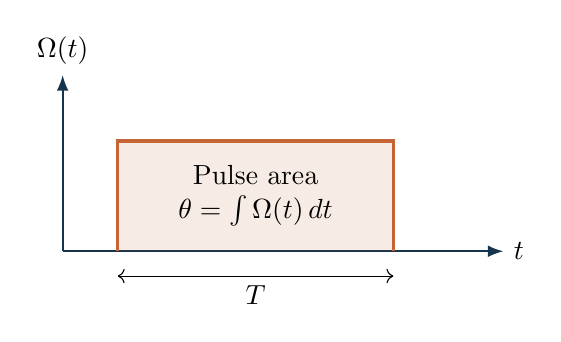
\begin{tikzpicture}[x=.7cm,y=.7cm]
    \draw[flow] (0,0)--(8,0) node[right] {$t$};
    \draw[flow] (0,0)--(0,3.2) node[above] {$\Omega(t)$};
    \draw[Orange,very thick] (1,0)--(1,2)--(6,2)--(6,0);
    \fill[Orange,opacity=.13] (1,0) rectangle (6,2);
    \draw[<->] (1,-.45)--(6,-.45) node[midway,below] {$T$};
    \node[align=center] at (3.5,1) {Pulse area\\$\theta=\int\Omega(t)\,dt$};
  \end{tikzpicture}\par
  \footnotesize Rectangular envelope 为解释示意；0918 的真实 envelope 未恢复。
  \column{.47\linewidth}
  \[
    P_1=\sin^2(\theta/2),\qquad \theta=\Omega T
  \]
  \small $\Omega$ 为 angular Rabi frequency。适用条件：initial $\ket0$、resonant drive、固定 rotation axis、理想 two-level dynamics。\par
  \textbf{Amplitude Rabi}：固定 $T$，改变 strength。\par
  \textbf{Time Rabi}：固定 strength，改变 $T$。\par
  $\pi$ pulse 是 $180^\circ$ state rotation；$\pi/2$ pulse 可产生等 population superposition。
  \end{columns}
  \vspace{2mm}
  \takeaway{0918 扫的是 drive-amplitude setting；readout magnitude 不是直接的 $P_1$。}
  \small 稳定 two-state readout 下，averaged IQ 可近似沿两端点连线；取 magnitude / phase 后一般不再是简单 sinusoid。
  \src{Krantz Eqs. (92)--(94)，p. 29 \cite{krantz}；0918 Rabi CSV。}
\end{frame}

\begin{frame}{T1 与 Ramsey：先理解 sequence，再选择 fit model}
  \begin{columns}[T]
  \column{.49\linewidth}
  \begin{block}{T1：excitation 的衰减}
    $\ket0\ \xrightarrow{\pi}\ \ket1\ \xrightarrow{\text{delay }t}\ \text{readout}$
    \[
      P_1(t)=B+A e^{-t/T_1}.
    \]
    $A$ 为 initial contrast，$B$ 为 long-delay baseline。\par
    $t=T_1$ 时，\textbf{相对 baseline 的 excess} 变为原来的 $1/e$。
  \end{block}
  \column{.49\linewidth}
  \begin{block}{Ramsey：relative phase 的保持}
    $\ket0\ \xrightarrow{\pi/2}\ \text{superposition}\ \xrightarrow{t}\ \pi/2\ \to\ \text{readout}$
    \[
      P_1(t)=B+A e^{-t/T_2^*}\cos(2\pi f_Rt+\phi).
    \]
    第二个 pulse 将 relative phase 转成 population contrast。\par
    $f_R$ 是 fringe frequency，不是 carrier frequency。
  \end{block}
  \end{columns}
  \small
  等 population superposition：$(\ket0+e^{i\phi}\ket1)/\sqrt2$；amplitudes 的大小是 $1/\sqrt2$，probabilities 是 $1/2$。\par
  Stationary exponential relaxation / dephasing 下，$1/T_2=1/(2T_1)+1/T_\phi$；不能将无关 runs 的 $T_1,T_2^*$ 任意代入比较。
  \src{Krantz Fig. 5、Sec. III.B.2--3，pp. 13--16 \cite{krantz}。}
\end{frame}

\begin{frame}{Readout calibration：prepare state 与 assign state 不同}
  \begin{columns}[T]
  \column{.49\linewidth}
  \begin{block}{Preparation}
    Without $\pi$：名义上 prepare $\ket0$。\par
    With $\pi$：名义上 prepare $\ket1$。\par
    这些 labels 记录的是\textbf{执行的操作}，不是每个 shot 的真实 state 保证。
  \end{block}
  \column{.49\linewidth}
  \begin{block}{Assignment}
    根据测得的 $(I,Q)$，classifier 输出 0 或 1。\par
    GMM clustering 本身不能给 cluster 赋予物理 state label；需要 preparation reference。
  \end{block}
  \end{columns}
  \[
    F_0=P(\mathrm{assign}\ 0\mid\mathrm{nominal\ prepare}\ 0),\quad
    F_1=P(\mathrm{assign}\ 1\mid\mathrm{nominal\ prepare}\ 1),\quad
    F_{\mathrm{bal}}=\frac{F_0+F_1}{2}.
  \]
  \small
  本报告使用现有 audit 的 \textbf{held-out linear classifier}：在一半 records 上训练，在另一半评估，再交换。\par
  该 accuracy 包含 preparation / relaxation 影响；不是原始 GMM estimator 的复现，也不是 isolated measurement error。
  \src{Krantz Sec. V.C；Blais Sec. V.C.2 \cite{krantz,blais}；audit\_raw\_physics.py 的 readout()。}
\end{frame}

\section{从数据判断可信度}
\begin{frame}{如何阅读对照页：review flag 不等于实验测错}
  \begin{columns}[T]
  \column{.49\linewidth}
  \textbf{三种证据强度}\par
  \begin{enumerate}
    \item \textbf{Observation}：flat trace、overlap、edge、scatter。
    \item \textbf{Model diagnostic}：fit score、resolution、coverage、residual。
    \item \textbf{Possible cause}：需要进一步实验区分，不能直接当作事实。
  \end{enumerate}
  \small Reference 表示相对清晰；不意味着已完成 calibration certification。不同 case 通常不是 controlled pair。
  \column{.49\linewidth}
  \textbf{本报告使用的 diagnostic}\par
  {\small $R^2$：coefficient of determination。}\par
  \[
    R^2=1-\frac{\sum_i(y_i-\hat y_i)^2}{\sum_i(y_i-\bar y)^2}.
  \]
  \small $y_i$ 为观察，$\hat y_i$ 为 model prediction，$\bar y$ 为 mean。\par
  Residual $r_i=y_i-\hat y_i$；相邻 correlation 反映 model 未解释的有序结构。\par
  FWHM = Full Width at Half Maximum。\par
  a.u. = arbitrary units；图中无 absolute gain calibration。
  \end{columns}
  \vspace{1mm}
  \takeaway{46 个 flagged cases + 1 个 resonator review case = 47 个案例；全部附图并给出验证方向。}
  \src{Hash-verified recorded review；本地 $R^2<0.8$ 等规则仅用于筛查，不是 universal threshold 或 significance test。}
\end{frame}

\begin{frame}[t,label=case-t1-004]{T1 Visibility / 004}{Flat trace 不能确定一个很长的 T1}
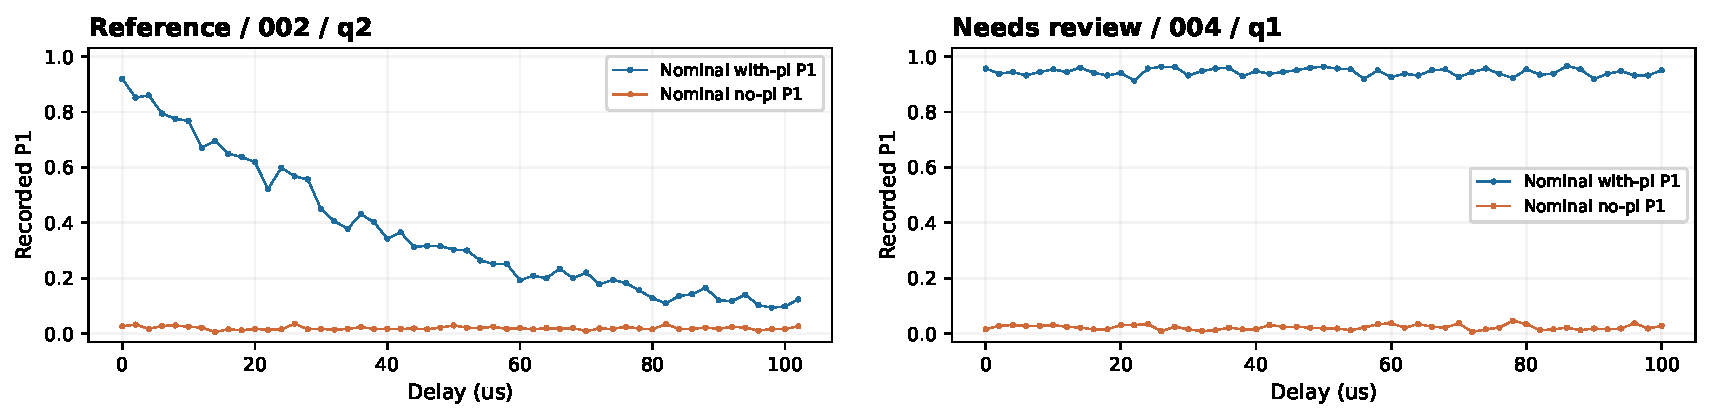
\includegraphics[width=\linewidth]{figures/t1-004.pdf}
\vspace{-1.5mm}
{\fontsize{8.4}{10}\selectfont\color{Muted} Contrast fit: $R^2=0.008$; lifetime reaches $10000\,\mu s$ fit bound; lifetime unresolved\par}
\vspace{1mm}{\fontsize{8.7}{10.4}\selectfont\renewcommand{\arraystretch}{1.08}\begin{tabularx}{\linewidth}{@{}>{\bfseries\color{Navy}}p{1.35cm}X@{}}
观察 & Nominal with-pi P1：0.956 $\to$ 0.950（0--100 us）；几乎没有 resolved decay。 \\
可能原因 & Lifetime 超出窗口；delay 未实际改变；readout 前重激发；channel 或 acquisition 有误。 \\
验证 & 核对 executed sequence 与 time units；重复 preparation reference，再扩大 delay window。
\end{tabularx}}
\vfill
{\fontsize{6.5}{8}\selectfont\color{Muted} Source: 0918 / T1 Visibility / 002, 004; raw CSV replotted. P1 channel preparation order inferred; metrics fit contrast.\par}
\end{frame}

\begin{frame}[t,label=case-readout-008]{GMM Readout Clusters / 008}{Preparation label 不等于可可靠区分的 state}
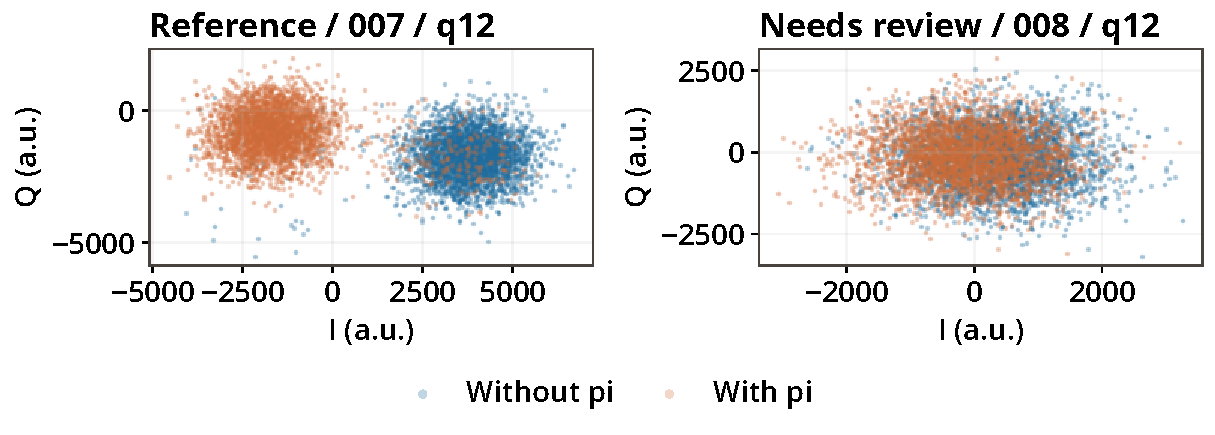
\includegraphics[width=\linewidth]{figures/readout-008.pdf}
\vspace{-1.5mm}
{\fontsize{8.4}{10}\selectfont\color{Muted} Held-out linear classifier: balanced accuracy $61.70\%$; not original GMM fidelity\par}
\vspace{1mm}{\fontsize{8.7}{10.4}\selectfont\renewcommand{\arraystretch}{1.08}\begin{tabularx}{\linewidth}{@{}>{\bfseries\color{Navy}}p{1.35cm}X@{}}
观察 & Held-out linear balanced accuracy = 61.70\%；nominal preparation groups 重叠。 \\
可能原因 & Preparation pulse 不准；probe setting 不合适；measurement 期间 relaxation；measurement chain noise。 \\
验证 & 先验证 preparation / Rabi，再检查 probe frequency、integration window 和 demodulated time trace。
\end{tabularx}}
\vfill
{\fontsize{6.5}{8}\selectfont\color{Muted} Source: 0918 / GMM Readout Clusters / 007, 008; raw CSV replotted. Classifier predicts preparation labels; not isolated readout error.\par}
\end{frame}

\begin{frame}[t,label=case-rabi-003]{Rabi Oscillation / 003}{Noise-like trace 中，fitter 仍然会返回 period}
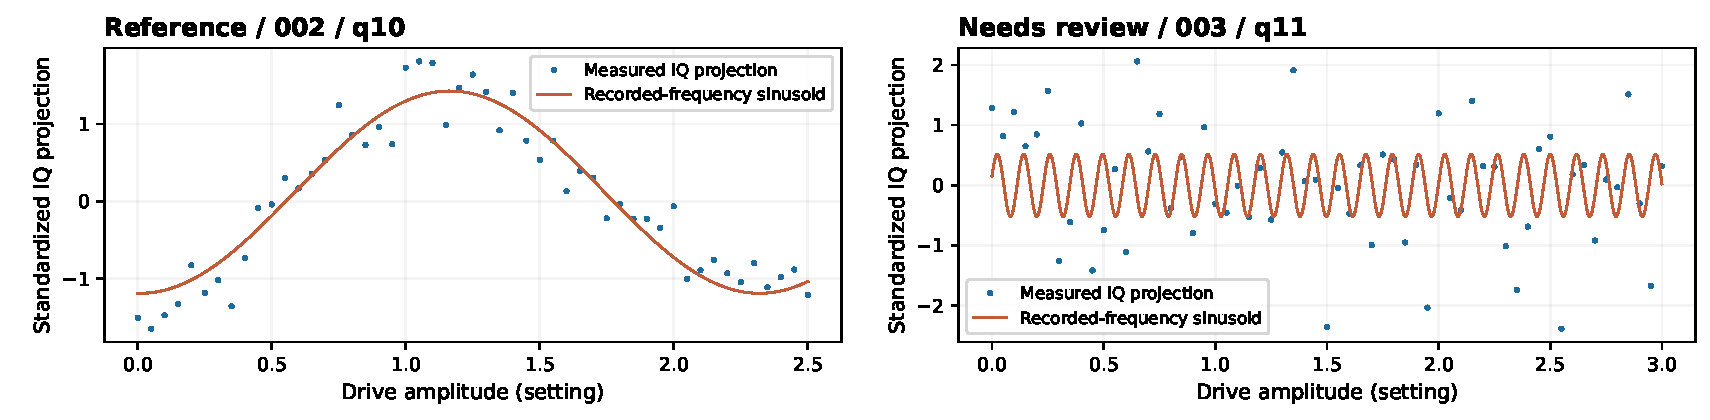
\includegraphics[width=\linewidth]{figures/rabi-003.pdf}
\vspace{-1.5mm}
{\fontsize{8.4}{10}\selectfont\color{Muted} IQ-projection fit: $R^2=0.130$; coverage $25.44$ cycles; $2.4$ samples/cycle\par}
\vspace{1mm}{\fontsize{8.7}{10.4}\selectfont\renewcommand{\arraystretch}{1.08}\begin{tabularx}{\linewidth}{@{}>{\bfseries\color{Navy}}p{1.35cm}X@{}}
观察 & 没有清晰完整 cycle；R2=0.130；每个 fitted cycle 仅 2.36 个 samples。 \\
可能原因 & Drive / readout contrast 不足、frequency 不准或 pulse path 问题；candidate 高频也可能是 noise fitting。 \\
验证 & 先验证 spectroscopy 与 readout，再重复 sweep；不能直接采用 fitted half-period 作为 pi amplitude。
\end{tabularx}}
\vfill
{\fontsize{6.5}{8}\selectfont\color{Muted} Source: 0918 / Rabi Oscillation / 002, 003; raw CSV replotted. IQ projection is standardized independently; its sign is arbitrary.\par}
\end{frame}

\begin{frame}[t,label=case-rabi-007]{Rabi Oscillation / 007}{高 fit score 不保证 period 已被测到}
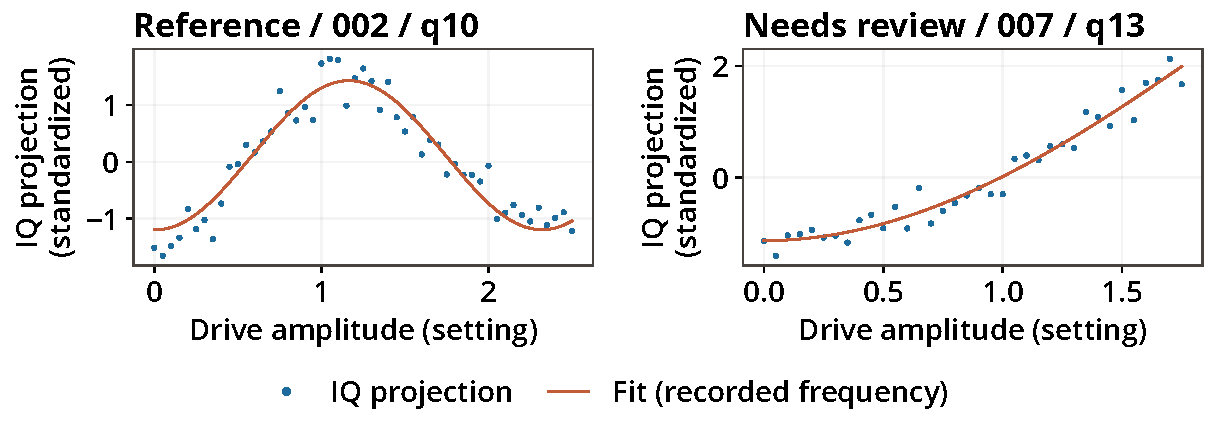
\includegraphics[width=\linewidth]{figures/rabi-007.pdf}
\vspace{-1.5mm}
{\fontsize{8.4}{10}\selectfont\color{Muted} IQ-projection fit: $R^2=0.959$; coverage $0.22$ cycles; $159.7$ samples/cycle\par}
\vspace{1mm}{\fontsize{8.7}{10.4}\selectfont\renewcommand{\arraystretch}{1.08}\begin{tabularx}{\linewidth}{@{}>{\bfseries\color{Navy}}p{1.35cm}X@{}}
观察 & Scan 仅覆盖 candidate cycle 的 0.22；period 很大部分来自 extrapolation。 \\
可能原因 & Amplitude window 太短；局部 response 被误当作完整 sinusoid；模型可辨识性不足。 \\
验证 & 在合适的控制范围内扩大 amplitude scan；观察 turning point 与 return；验证 pi endpoint。
\end{tabularx}}
\vfill
{\fontsize{6.5}{8}\selectfont\color{Muted} Source: 0918 / Rabi Oscillation / 002, 007; raw CSV replotted. IQ projection is standardized independently; its sign is arbitrary.\par}
\end{frame}

\begin{frame}[t,label=case-spectroscopy-008]{Qubit Spectroscopy / 008}{Scan boundary 限制了 resonance center 的判断}
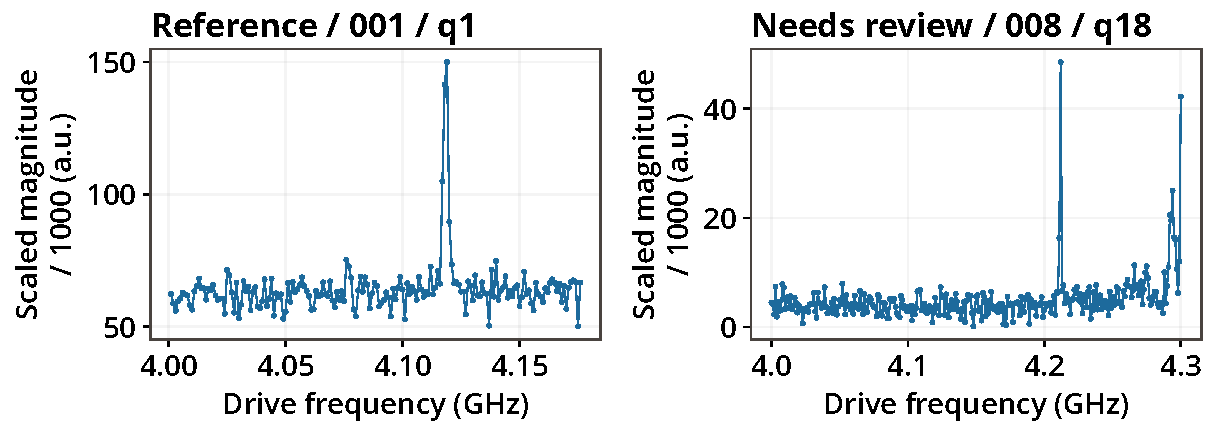
\includegraphics[width=\linewidth]{figures/spectroscopy-008.pdf}
\vspace{-1.5mm}
{\fontsize{8.4}{10}\selectfont\color{Muted} IQ single-line diagnostic: $R^2=0.312$; step $1.00$ MHz; FWHM $13.30$ MHz\par}
\vspace{1mm}{\fontsize{8.7}{10.4}\selectfont\renewcommand{\arraystretch}{1.08}\begin{tabularx}{\linewidth}{@{}>{\bfseries\color{Navy}}p{1.35cm}X@{}}
观察 & Candidate center=4.300 GHz 位于 scan 边界；不能完整观察两侧 response。 \\
可能原因 & Feature 延伸到窗口外、多个 transitions 或 baseline 变化；边界值不是已测定的 center。 \\
验证 & 扩大 frequency window 观察两侧；检查 candidate feature 的复现性与 drive-strength dependence。
\end{tabularx}}
\vfill
{\fontsize{6.5}{8}\selectfont\color{Muted} Source: 0918 / Qubit Spectroscopy / 001, 008; raw CSV replotted. Magnitude plotted; reported R2 and FWHM are from IQ-projection diagnostic.\par}
\end{frame}

\begin{frame}[t,label=case-spectroscopy-005]{Qubit Spectroscopy / 005}{Fit score 不能补足 frequency resolution}
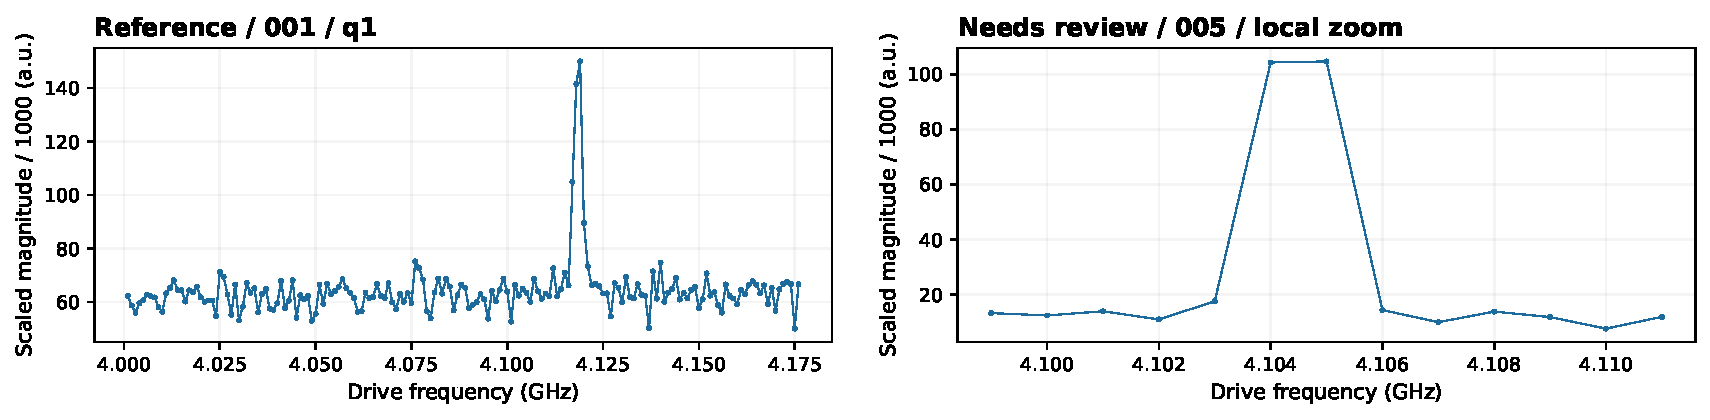
\includegraphics[width=\linewidth]{figures/spectroscopy-005.pdf}
\vspace{-1.5mm}
{\fontsize{8.4}{10}\selectfont\color{Muted} IQ single-line diagnostic: $R^2=0.965$; step $1.00$ MHz; FWHM $0.50$ MHz\par}
\vspace{1mm}{\fontsize{8.7}{10.4}\selectfont\renewcommand{\arraystretch}{1.08}\begin{tabularx}{\linewidth}{@{}>{\bfseries\color{Navy}}p{1.35cm}X@{}}
观察 & Frequency step=1.00 MHz，candidate FWHM=0.50 MHz；采样不足。 \\
可能原因 & 实际窄 resonance 或 isolated outlier；现有 grid 无法可靠区分，也不支持过高 linewidth precision。 \\
验证 & 在 feature 附近使用更小 frequency step，并重复采样；比较 peak / dip 的宽度与 reproducibility。
\end{tabularx}}
\vfill
{\fontsize{6.5}{8}\selectfont\color{Muted} Source: 0918 / Qubit Spectroscopy / 001, 005; raw CSV replotted. Magnitude plotted; reported R2 and FWHM are from IQ-projection diagnostic.\par}
\end{frame}

\begin{frame}[t,label=case-ramsey-008]{T2 Ramsey / 008}{Envelope 结构超出单一 exponential model}
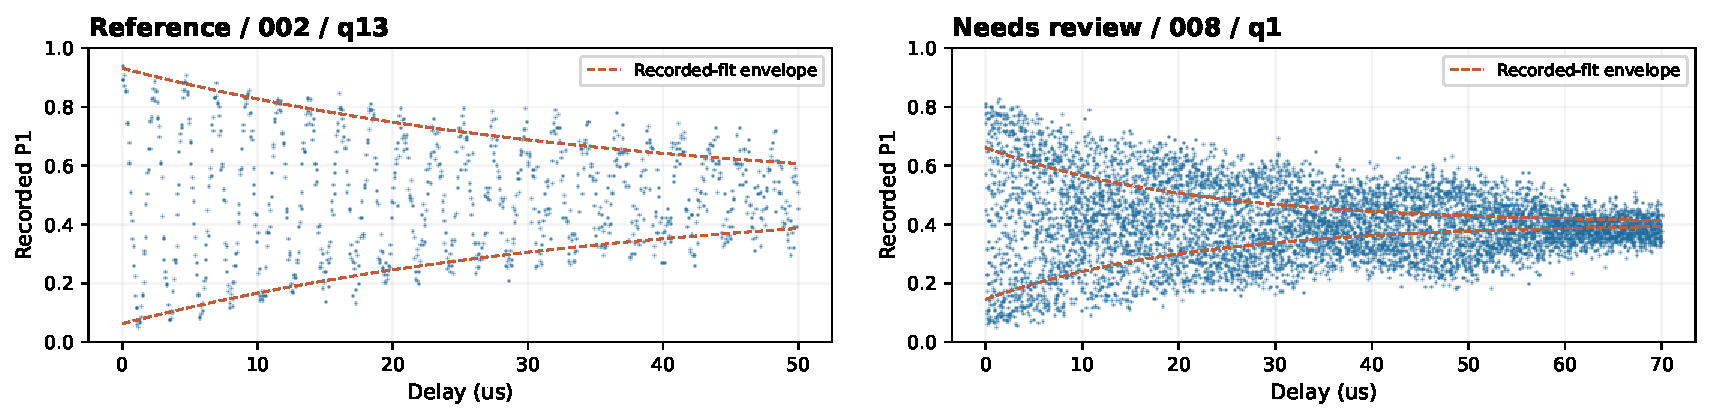
\includegraphics[width=\linewidth]{figures/ramsey-008.pdf}
\vspace{-1.5mm}
{\fontsize{8.4}{10}\selectfont\color{Muted} Recorded Ramsey fit: $R^2=0.328$; candidate $T_2^*=21.78\,\mu s$; residual correlation $0.38$\par}
\vspace{1mm}{\fontsize{8.7}{10.4}\selectfont\renewcommand{\arraystretch}{1.08}\begin{tabularx}{\linewidth}{@{}>{\bfseries\color{Navy}}p{1.35cm}X@{}}
观察 & Dense oscillation trace 在约 40--50 us 重新变宽；single-envelope fit 不能覆盖全部结构。 \\
可能原因 & Multiple frequencies / beating、drift 或 readout / noise 变化；不能仅凭图确认 low-frequency noise。 \\
验证 & 检查 cycle-resolved trace 与 residual；重复 acquisition；比较 fit window、envelope 与 echo。
\end{tabularx}}
\vfill
{\fontsize{6.5}{8}\selectfont\color{Muted} Source: 0918 / T2 Ramsey / 002, 008; raw CSV replotted. Reference also flagged; envelope shown, not the full fitted oscillation.\par}
\end{frame}

\begin{frame}[t,label=case-resonator-006]{Resonator Spectroscopy / 006}{First-point spike 是 resonance 还是 acquisition transient？}
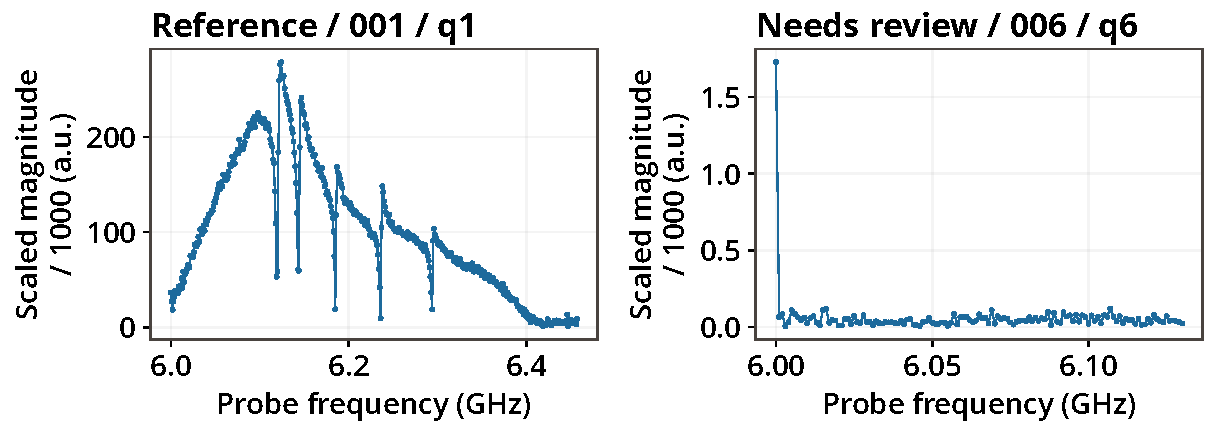
\includegraphics[width=\linewidth]{figures/resonator-006.pdf}
\vspace{-1.5mm}
{\fontsize{8.4}{10}\selectfont\color{Muted} Descriptive screen only: window 6.000--6.130 GHz; no validated transfer-function fit\par}
\vspace{1mm}{\fontsize{8.7}{10.4}\selectfont\renewcommand{\arraystretch}{1.08}\begin{tabularx}{\linewidth}{@{}>{\bfseries\color{Navy}}p{1.35cm}X@{}}
观察 & Scaled magnitude 首点约 1728，次点约 66，后续 median 约 41；窗口内无 resolved interior resonance。 \\
可能原因 & Settling / acquisition discontinuity、edge / out-of-window resonance，或 useful signal 不足。 \\
验证 & 加入 settling 后重测首点；反向 sweep；扩大窗口并同时检查 phase / IQ。
\end{tabularx}}
\vfill
{\fontsize{6.5}{8}\selectfont\color{Muted} Source: 0918 / Resonator Spectroscopy / 001, 006; raw CSV replotted. Independent scales/settings; multiple features can be normal.\par}
\end{frame}


\begin{frame}{判断一个 calibration number 前，依次检查什么？}
  \small
  \begin{tabularx}{\linewidth}{@{}p{2.5cm}Xp{4.5cm}@{}}
  \toprule
  层次 & 要检查的问题 & 0918 例子 \\
  \midrule
  Observable & 记录的是 IQ、magnitude 还是 population？ & Rabi magnitude 不直接等于 $P_1$ \\
  Coverage & 两侧 feature / 足够 cycle / 足够 decay 是否出现？ & Spectroscopy/008；Rabi/007；T1/004 \\
  Resolution & Frequency / delay / amplitude step 是否足够？ & Spectroscopy/005 \\
  Model adequacy & Residual 是否有结构？模型是否过于简单？ & Ramsey/008；多个 Rabi cases \\
  Preparation / readout & Reference groups 是否能可靠区分？ & GMM/008 \\
  Reproducibility & 重复或改变 sweep direction 后是否一致？ & Resonator/006 的 first-point spike \\
  \bottomrule
  \end{tabularx}
  \vspace{1mm}
  \takeaway{Fit 返回数值只是开始；parameter 是否被数据约束、能否用于目标操作，需要单独判断。}
  \src{本报告对 0918 recorded evidence 的解释归纳；possible causes 尚未经 intervention 验证。}
\end{frame}

\section{References 与来源}
\begin{frame}{References：hardware、control、readout 的理论依据}
  \begin{thebibliography}{B}
  \bibitem[K]{krantz} P. Krantz et al.\par
  \emph{A Quantum Engineer's Guide to Superconducting Qubits}.\par
  Applied Physics Reviews \textbf{6}, 021318 (2019).\par
  \href{https://doi.org/10.1063/1.5089550}{doi:10.1063/1.5089550}\par
  \footnotesize Local source: arXiv:1904.06560v5（2021 revision）。\par
  Fig. 1：Transmon；Fig. 5：T1 / Ramsey；Eqs. (92)--(94)：rotation；Fig. 22：IQ chain。
  \bibitem[B]{blais} A. Blais, A. L. Grimsmo, S. M. Girvin, and A. Wallraff.\par
  \emph{Circuit Quantum Electrodynamics}.\par
  Reviews of Modern Physics \textbf{93}, 025005 (2021).\par
  \href{https://doi.org/10.1103/RevModPhys.93.025005}{doi:10.1103/RevModPhys.93.025005}\par
  \footnotesize Local source: arXiv:2005.12667v1（2020）。\par
  Figs. 14、16：measurement chain；Eq. (107)、Fig. 19：dispersive response。
  \end{thebibliography}
\end{frame}

\begin{frame}{Data provenance 与解释边界}
  \begin{itemize}
    \item \textbf{Measurements}：0918 raw CSV，共 64 cases。对照图均从 numeric arrays 重绘；没有采集新实验。
    \item \textbf{Diagnostics}：复用已完成的 recorded audit。制作时核对全部输入、报告和 audit script 的 SHA-256（Secure Hash Algorithm 256-bit）checksums。
    \item \textbf{Estimator}：T1 指标 fit contrast；Rabi 指标 fit projected IQ；spectroscopy 的 $R^2$ 与 FWHM 来自 single-Lorentzian IQ diagnostic。
    \item \textbf{Boundaries}：未确认 shot counts / noise covariance；未复现原 GMM estimator；resonator 未完成完整 circuit transfer-function fit。
    \item \textbf{Possible causes} 是待验证解释；raw constraints 通过，不保证 acquisition 或 causal interpretation 正确。
  \end{itemize}
  \vspace{2mm}
  \small
  随附 \texttt{evidence.json} 保存 source / hash / metrics / policy；\texttt{coverage.md} 列出 47 个 case；\texttt{data/} 包含可重绘的 numeric snapshots。\par
  Notes 与 reference PDFs 位于本 slides 的上级 discussion；source annotations 记录 consulted version 与 passages。
\end{frame}

\ifdefined\MainOnly
\else
\appendix
\section{Appendix：完整案例}
\begin{frame}[label=case-index]{完整案例导航：47 个 review cases}
  \footnotesize\setlength{\parskip}{.6mm}
  以下 case buttons 可跳转；带 * 的 8 个案例已在正文展示，其余 39 个位于附录。\par
  \textbf{T1 Visibility} (3)\par \hyperlink{case-t1-001}{\beamerbutton{001}} \hyperlink{case-t1-004}{\beamerbutton{004*}} \hyperlink{case-t1-005}{\beamerbutton{005}}\par\vspace{1mm}
\textbf{T2 Ramsey} (8)\par \hyperlink{case-ramsey-001}{\beamerbutton{001}} \hyperlink{case-ramsey-002}{\beamerbutton{002}} \hyperlink{case-ramsey-003}{\beamerbutton{003}} \hyperlink{case-ramsey-004}{\beamerbutton{004}} \hyperlink{case-ramsey-005}{\beamerbutton{005}} \hyperlink{case-ramsey-006}{\beamerbutton{006}} \hyperlink{case-ramsey-007}{\beamerbutton{007}} \hyperlink{case-ramsey-008}{\beamerbutton{008*}}\par\vspace{1mm}
\textbf{Rabi Oscillation} (15)\par \hyperlink{case-rabi-001}{\beamerbutton{001}} \hyperlink{case-rabi-003}{\beamerbutton{003*}} \hyperlink{case-rabi-004}{\beamerbutton{004}} \hyperlink{case-rabi-005}{\beamerbutton{005}} \hyperlink{case-rabi-006}{\beamerbutton{006}} \hyperlink{case-rabi-007}{\beamerbutton{007*}} \hyperlink{case-rabi-008}{\beamerbutton{008}} \hyperlink{case-rabi-009}{\beamerbutton{009}} \hyperlink{case-rabi-010}{\beamerbutton{010}} \hyperlink{case-rabi-011}{\beamerbutton{011}} \hyperlink{case-rabi-012}{\beamerbutton{012}} \hyperlink{case-rabi-013}{\beamerbutton{013}} \hyperlink{case-rabi-014}{\beamerbutton{014}} \hyperlink{case-rabi-015}{\beamerbutton{015}} \hyperlink{case-rabi-016}{\beamerbutton{016}}\par\vspace{1mm}
\textbf{Qubit Spectroscopy} (15)\par \hyperlink{case-spectroscopy-002}{\beamerbutton{002}} \hyperlink{case-spectroscopy-004}{\beamerbutton{004}} \hyperlink{case-spectroscopy-005}{\beamerbutton{005*}} \hyperlink{case-spectroscopy-006}{\beamerbutton{006}} \hyperlink{case-spectroscopy-007}{\beamerbutton{007}} \hyperlink{case-spectroscopy-008}{\beamerbutton{008*}} \hyperlink{case-spectroscopy-009}{\beamerbutton{009}} \hyperlink{case-spectroscopy-011}{\beamerbutton{011}} \hyperlink{case-spectroscopy-012}{\beamerbutton{012}} \hyperlink{case-spectroscopy-013}{\beamerbutton{013}} \hyperlink{case-spectroscopy-014}{\beamerbutton{014}} \hyperlink{case-spectroscopy-015}{\beamerbutton{015}} \hyperlink{case-spectroscopy-016}{\beamerbutton{016}} \hyperlink{case-spectroscopy-017}{\beamerbutton{017}} \hyperlink{case-spectroscopy-018}{\beamerbutton{018}}\par\vspace{1mm}
\textbf{GMM Readout Clusters} (5)\par \hyperlink{case-readout-002}{\beamerbutton{002}} \hyperlink{case-readout-003}{\beamerbutton{003}} \hyperlink{case-readout-004}{\beamerbutton{004}} \hyperlink{case-readout-005}{\beamerbutton{005}} \hyperlink{case-readout-008}{\beamerbutton{008*}}\par\vspace{1mm}
\textbf{Resonator Spectroscopy} (1)\par \hyperlink{case-resonator-006}{\beamerbutton{006*}}\par\vspace{1mm}

  \vfill
  \footnotesize Case ID 在每个 family 内独立编号。Resonator/006 是人工选出的 descriptive review case；其余 46 个来自现有 screen flags。
\end{frame}

\begin{frame}{附录阅读约定：Reference 与 Needs review}
  \begin{itemize}
    \item 每页只讨论一个 experiment family 的一个 review case；左图使用同 family 的较清晰 reference。
    \item Ramsey 全部 cases 均有 flag，因此使用相对清晰的 002 或 006，不能称为无缺陷的 normal standard。
    \item GMM/002--005 使用同为 q10 的 009；GMM/008 使用同为 q12 的 007。相同 qubit 仍不代表所有 settings 相同。
    \item 对 spectroscopy：图显示 magnitude；旁列指标来自 IQ-projection diagnostic，不能解释成同一个 observable 的 fit score。
    \item Rabi projection 的正负方向与 scale 是数学选择；不能把 standardized ordinate 直接当作 population。
    \item Threshold、fit range 与 model assumptions 影响 flags；不把 flag 数量解释成 failure rate。
  \end{itemize}
  \vspace{2mm}
  \hyperlink{case-index}{\beamerbutton{返回完整案例导航}}
\end{frame}

\begin{frame}[t,label=case-t1-001]{基线的选择影响衰减时间}{T1 Visibility / 001}
\setlength{\parskip}{0pt}
\begingroup
\setlength{\topsep}{0pt}\setlength{\partopsep}{0pt}
\begin{figure}
\centering
{\small
\makebox[.49\linewidth][c]{\textcolor{Teal}{左：基线选择下的时间常数较接近}}%
\makebox[.49\linewidth][c]{\textcolor{Orange}{右：改变基线后时间常数变化}}\par
}
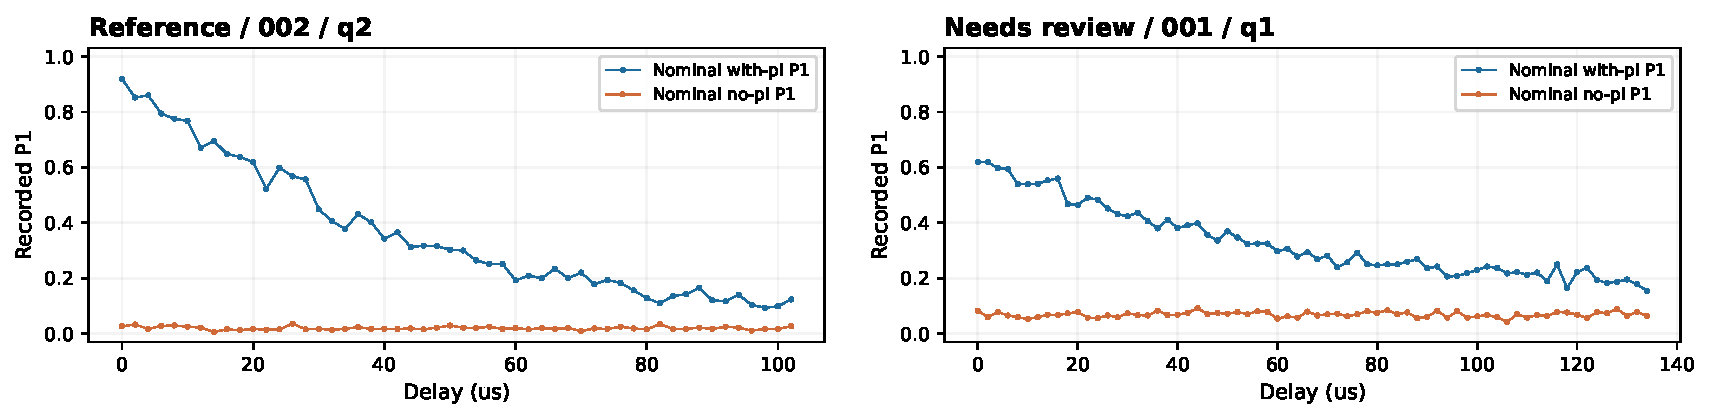
\includegraphics[width=\linewidth,height=34mm,keepaspectratio]{figures/t1-001.pdf}
\caption{左：对照 002；右：案例 001。两路布居差拟合： $\tau_{free}=55.94$ / $\tau_0=77.48\,\mu s$。准备顺序为推断；拟合对象是两路布居差。}
\label{fig-t1-001}
\end{figure}
\endgroup
{\small\textbf{判断：衰减时间依赖基线假设；需延长等待并检查参考通道。}\par}
\end{frame}

\begin{frame}[t,label=case-t1-005]{基线的选择影响衰减时间}{T1 Visibility / 005}
\setlength{\parskip}{0pt}
\begingroup
\setlength{\topsep}{0pt}\setlength{\partopsep}{0pt}
\begin{figure}
\centering
{\small
\makebox[.49\linewidth][c]{\textcolor{Teal}{左：基线选择下的时间常数较接近}}%
\makebox[.49\linewidth][c]{\textcolor{Orange}{右：改变基线后时间常数变化}}\par
}
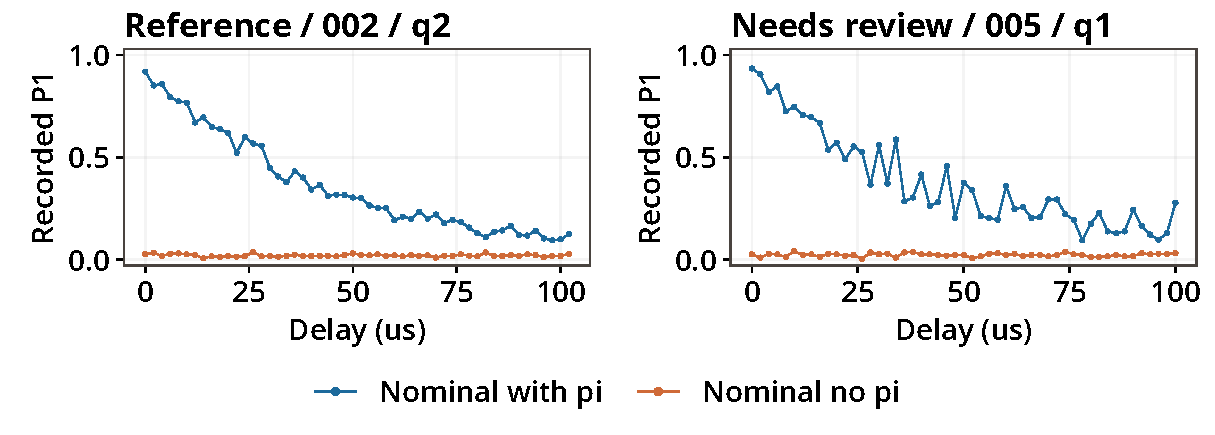
\includegraphics[width=\linewidth,height=34mm,keepaspectratio]{figures/t1-005.pdf}
\caption{左：对照 002；右：案例 005。两路布居差拟合： $\tau_{free}=33.01$ / $\tau_0=44.48\,\mu s$。准备顺序为推断；拟合对象是两路布居差。}
\label{fig-t1-005}
\end{figure}
\endgroup
{\small\textbf{判断：衰减时间依赖基线假设；需延长等待并检查参考通道。}\par}
\end{frame}

\begin{frame}[t,label=case-ramsey-001]{单一包络仍有未解释的结构}{T2 Ramsey / 001}
\setlength{\parskip}{0pt}
\begingroup
\setlength{\topsep}{0pt}\setlength{\partopsep}{0pt}
\begin{figure}
\centering
{\small
\makebox[.49\linewidth][c]{\textcolor{Teal}{左：较清晰的振荡也有相关残差}}%
\makebox[.49\linewidth][c]{\textcolor{Orange}{右：当前模型对记录的解释不足}}\par
}
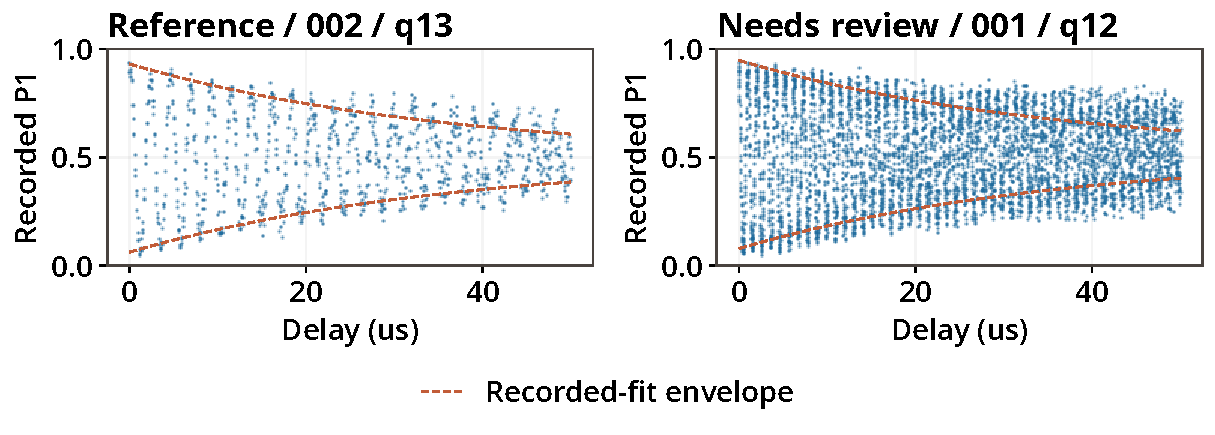
\includegraphics[width=\linewidth,height=34mm,keepaspectratio]{figures/ramsey-001.pdf}
\caption{左：对照 002；右：案例 001。已有拟合： $R^2=0.769$；相邻残差相关系数 $0.10$。对照也有复查项；虚线仅表示包络，不是完整振荡预测。}
\label{fig-ramsey-001}
\end{figure}
\endgroup
{\small\textbf{判断：两侧均需复查；需比较拟合窗口与重复记录，不能只采纳时间常数。}\par}
\end{frame}

\begin{frame}[t,label=case-ramsey-002]{较清晰振荡也留下相关残差}{T2 Ramsey / 002}
\setlength{\parskip}{0pt}
\begingroup
\setlength{\topsep}{0pt}\setlength{\partopsep}{0pt}
\begin{figure}
\centering
{\small
\makebox[.49\linewidth][c]{\textcolor{Teal}{左：较清晰的振荡也有相关残差}}%
\makebox[.49\linewidth][c]{\textcolor{Orange}{右：当前模型仍留下相关残差}}\par
}
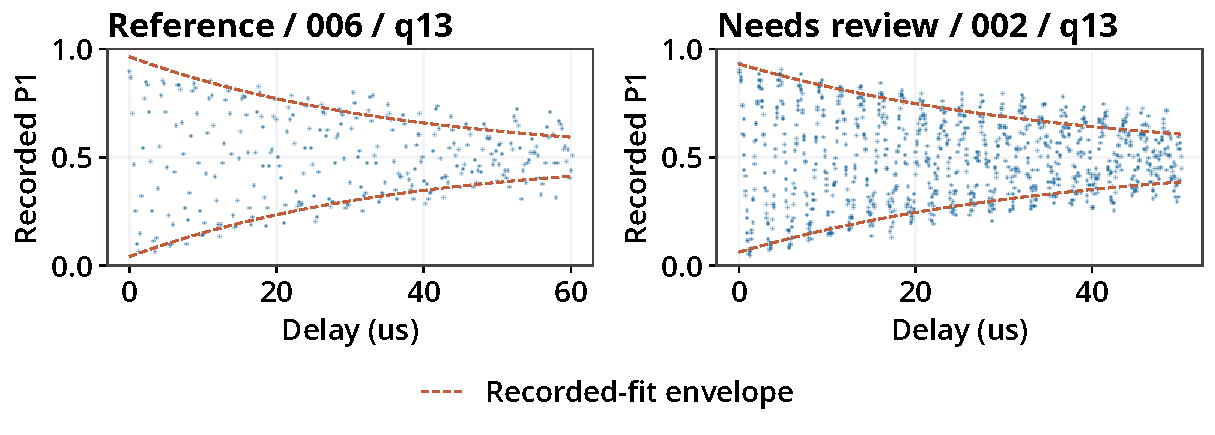
\includegraphics[width=\linewidth,height=34mm,keepaspectratio]{figures/ramsey-002.pdf}
\caption{左：对照 006；右：案例 002。已有拟合： $R^2=0.878$；相邻残差相关系数 $0.32$。对照也有复查项；虚线仅表示包络，不是完整振荡预测。}
\label{fig-ramsey-002}
\end{figure}
\endgroup
{\small\textbf{判断：两侧均需复查；需比较拟合窗口与重复记录，不能只采纳时间常数。}\par}
\end{frame}

\begin{frame}[t,label=case-ramsey-003]{单一包络仍有未解释的结构}{T2 Ramsey / 003}
\setlength{\parskip}{0pt}
\begingroup
\setlength{\topsep}{0pt}\setlength{\partopsep}{0pt}
\begin{figure}
\centering
{\small
\makebox[.49\linewidth][c]{\textcolor{Teal}{左：较清晰的振荡也有相关残差}}%
\makebox[.49\linewidth][c]{\textcolor{Orange}{右：当前模型仍留下相关残差}}\par
}
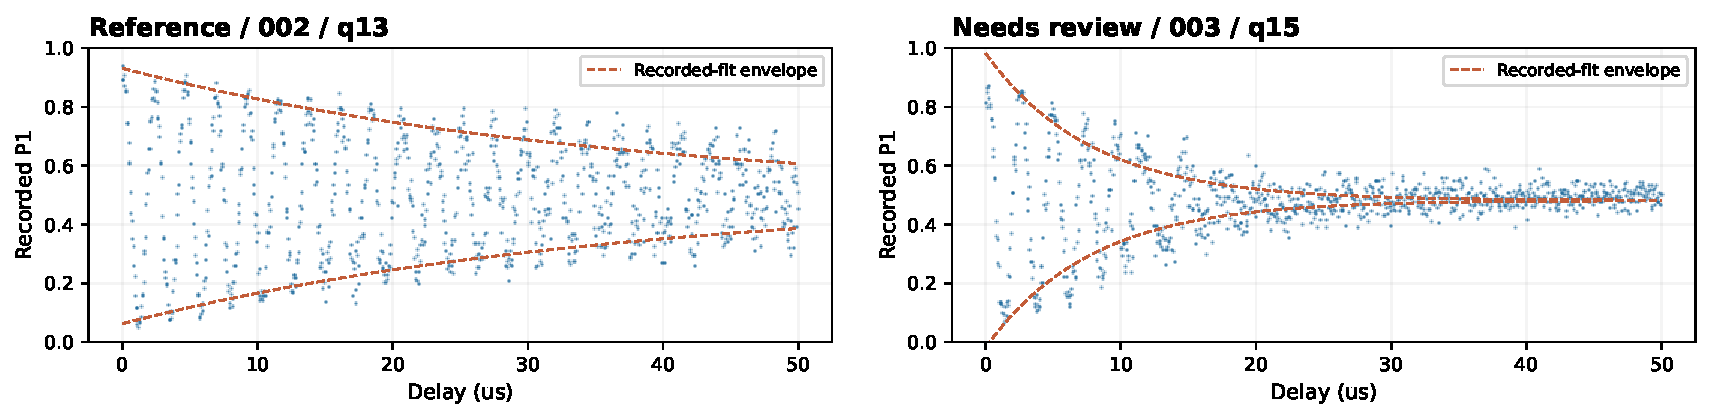
\includegraphics[width=\linewidth,height=34mm,keepaspectratio]{figures/ramsey-003.pdf}
\caption{左：对照 002；右：案例 003。已有拟合： $R^2=0.700$；相邻残差相关系数 $0.48$。对照也有复查项；虚线仅表示包络，不是完整振荡预测。}
\label{fig-ramsey-003}
\end{figure}
\endgroup
{\small\textbf{判断：两侧均需复查；需比较拟合窗口与重复记录，不能只采纳时间常数。}\par}
\end{frame}

\begin{frame}[t,label=case-ramsey-004]{单一包络仍有未解释的结构}{T2 Ramsey / 004}
\setlength{\parskip}{0pt}
\begingroup
\setlength{\topsep}{0pt}\setlength{\partopsep}{0pt}
\begin{figure}
\centering
{\small
\makebox[.49\linewidth][c]{\textcolor{Teal}{左：较清晰的振荡也有相关残差}}%
\makebox[.49\linewidth][c]{\textcolor{Orange}{右：当前模型对记录的解释不足}}\par
}
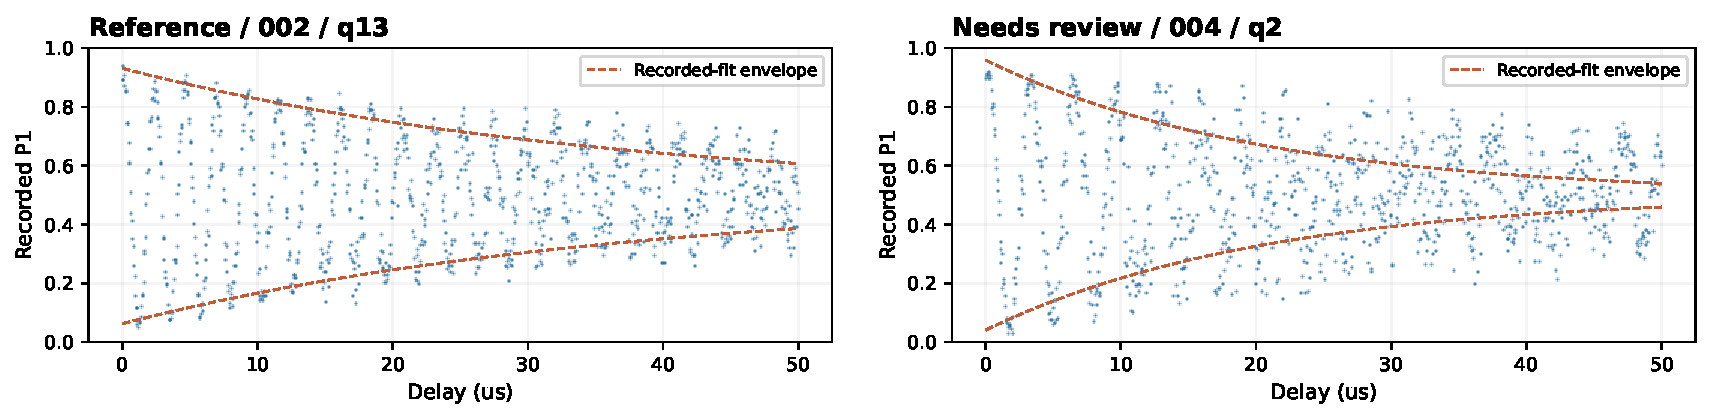
\includegraphics[width=\linewidth,height=34mm,keepaspectratio]{figures/ramsey-004.pdf}
\caption{左：对照 002；右：案例 004。已有拟合： $R^2=0.580$；相邻残差相关系数 $0.22$。对照也有复查项；虚线仅表示包络，不是完整振荡预测。}
\label{fig-ramsey-004}
\end{figure}
\endgroup
{\small\textbf{判断：两侧均需复查；需比较拟合窗口与重复记录，不能只采纳时间常数。}\par}
\end{frame}

\begin{frame}[t,label=case-ramsey-005]{单一包络仍有未解释的结构}{T2 Ramsey / 005}
\setlength{\parskip}{0pt}
\begingroup
\setlength{\topsep}{0pt}\setlength{\partopsep}{0pt}
\begin{figure}
\centering
{\small
\makebox[.49\linewidth][c]{\textcolor{Teal}{左：较清晰的振荡也有相关残差}}%
\makebox[.49\linewidth][c]{\textcolor{Orange}{右：当前模型对记录的解释不足}}\par
}
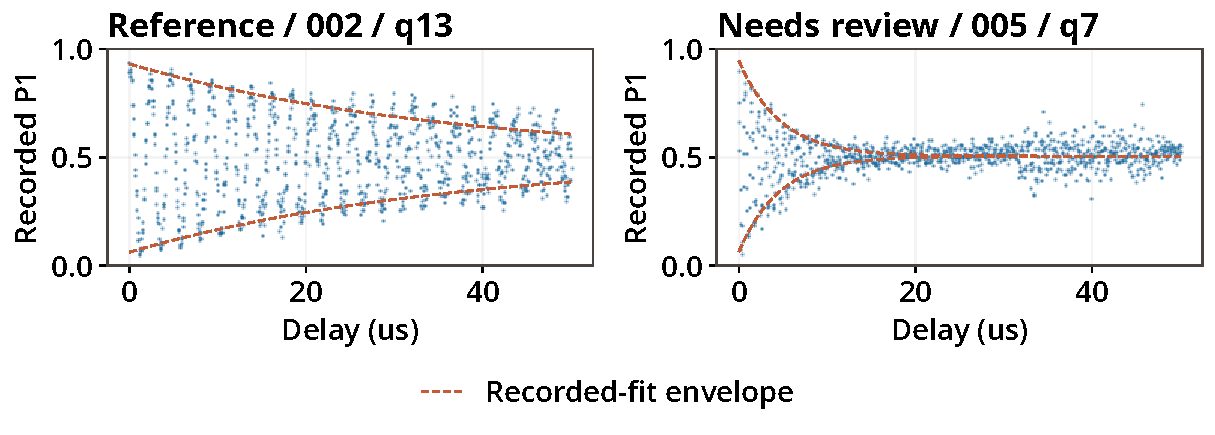
\includegraphics[width=\linewidth,height=34mm,keepaspectratio]{figures/ramsey-005.pdf}
\caption{左：对照 002；右：案例 005。已有拟合： $R^2=0.642$；相邻残差相关系数 $0.17$。对照也有复查项；虚线仅表示包络，不是完整振荡预测。}
\label{fig-ramsey-005}
\end{figure}
\endgroup
{\small\textbf{判断：两侧均需复查；需比较拟合窗口与重复记录，不能只采纳时间常数。}\par}
\end{frame}

\begin{frame}[t,label=case-ramsey-006]{较清晰振荡也留下相关残差}{T2 Ramsey / 006}
\setlength{\parskip}{0pt}
\begingroup
\setlength{\topsep}{0pt}\setlength{\partopsep}{0pt}
\begin{figure}
\centering
{\small
\makebox[.49\linewidth][c]{\textcolor{Teal}{左：较清晰的振荡也有相关残差}}%
\makebox[.49\linewidth][c]{\textcolor{Orange}{右：当前模型仍留下相关残差}}\par
}
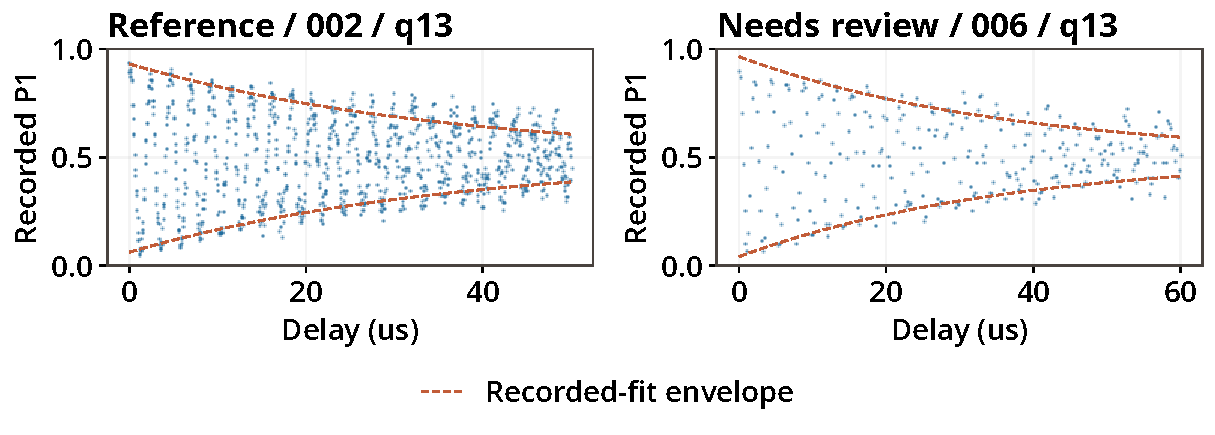
\includegraphics[width=\linewidth,height=34mm,keepaspectratio]{figures/ramsey-006.pdf}
\caption{左：对照 002；右：案例 006。已有拟合： $R^2=0.878$；相邻残差相关系数 $0.37$。对照也有复查项；虚线仅表示包络，不是完整振荡预测。}
\label{fig-ramsey-006}
\end{figure}
\endgroup
{\small\textbf{判断：两侧均需复查；需比较拟合窗口与重复记录，不能只采纳时间常数。}\par}
\end{frame}

\begin{frame}[t,label=case-ramsey-007]{单一包络仍有未解释的结构}{T2 Ramsey / 007}
\setlength{\parskip}{0pt}
\begingroup
\setlength{\topsep}{0pt}\setlength{\partopsep}{0pt}
\begin{figure}
\centering
{\small
\makebox[.49\linewidth][c]{\textcolor{Teal}{左：较清晰的振荡也有相关残差}}%
\makebox[.49\linewidth][c]{\textcolor{Orange}{右：当前模型仍留下相关残差}}\par
}
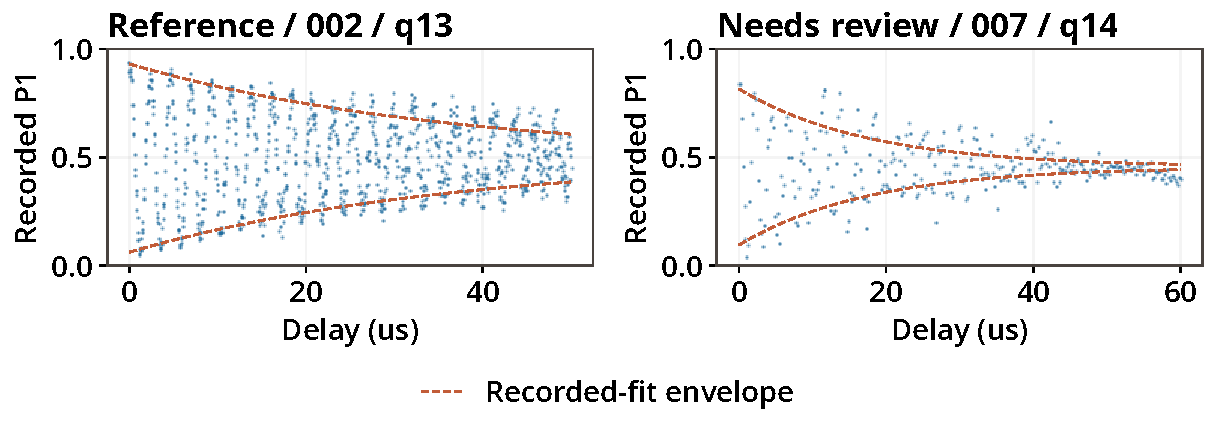
\includegraphics[width=\linewidth,height=34mm,keepaspectratio]{figures/ramsey-007.pdf}
\caption{左：对照 002；右：案例 007。已有拟合： $R^2=0.563$；相邻残差相关系数 $0.37$。对照也有复查项；虚线仅表示包络，不是完整振荡预测。}
\label{fig-ramsey-007}
\end{figure}
\endgroup
{\small\textbf{判断：两侧均需复查；需比较拟合窗口与重复记录，不能只采纳时间常数。}\par}
\end{frame}

\begin{frame}[t,label=case-rabi-001]{噪声状曲线也会返回拟合周期}{Rabi Oscillation / 001}
\setlength{\parskip}{0pt}
\begingroup
\setlength{\topsep}{0pt}\setlength{\partopsep}{0pt}
\begin{figure}
\centering
{\small
\makebox[.49\linewidth][c]{\textcolor{Teal}{左：转折与回返约束一个完整周期}}%
\makebox[.49\linewidth][c]{\textcolor{Orange}{右：散点不支持拟合的快速振荡}}\par
}
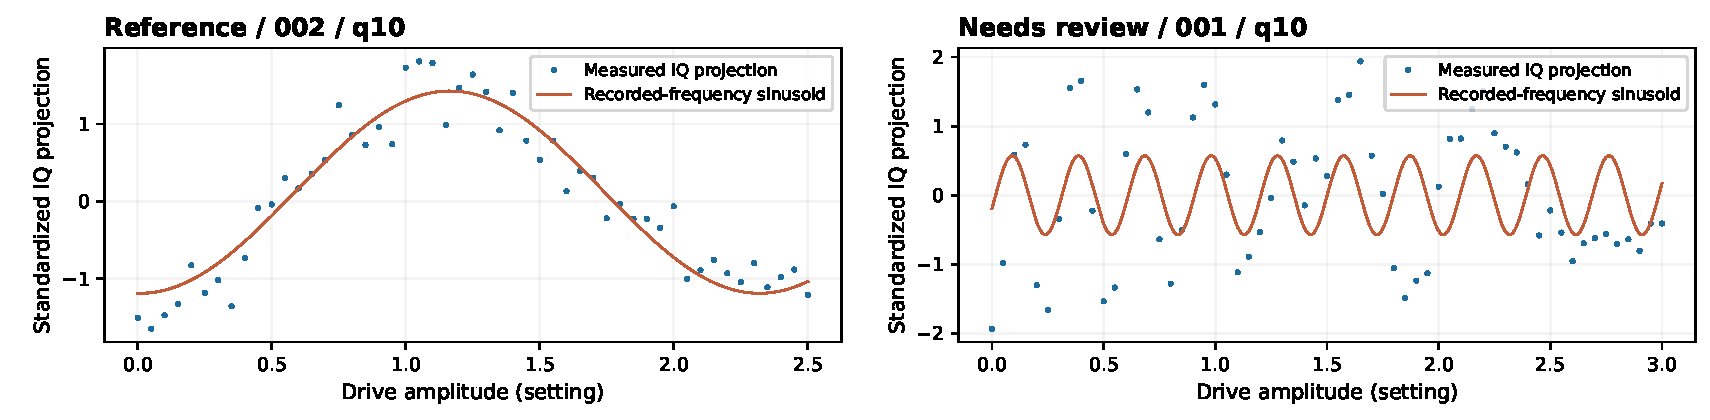
\includegraphics[width=\linewidth,height=34mm,keepaspectratio]{figures/rabi-001.pdf}
\caption{左：对照 002；右：案例 001。IQ 投影拟合： $R^2=0.160$；扫描覆盖 $10.10$ 个周期；每周期 $5.94$ 个采样点。IQ 投影独立标准化，符号与大小不可跨案例比较。}
\label{fig-rabi-001}
\end{figure}
\endgroup
{\small\textbf{判断：不能采用拟合半周期作为 $\pi$ 脉冲设置；需先恢复清晰振荡。}\par}
\end{frame}

\begin{frame}[t,label=case-rabi-004]{单一正弦模型仍有未解释的结构}{Rabi Oscillation / 004}
\setlength{\parskip}{0pt}
\begingroup
\setlength{\topsep}{0pt}\setlength{\partopsep}{0pt}
\begin{figure}
\centering
{\small
\makebox[.49\linewidth][c]{\textcolor{Teal}{左：转折与回返约束一个完整周期}}%
\makebox[.49\linewidth][c]{\textcolor{Orange}{右：正弦拟合仍留下结构性残差}}\par
}
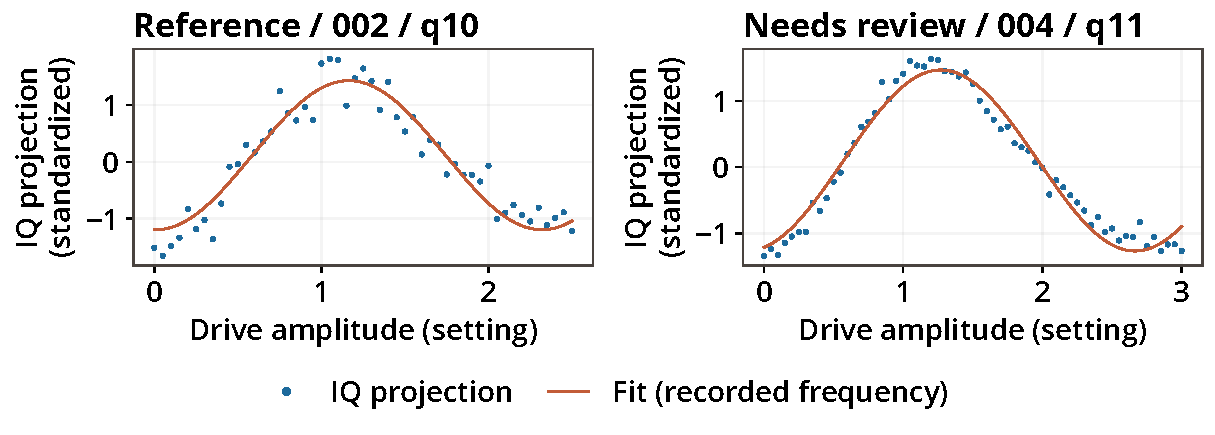
\includegraphics[width=\linewidth,height=34mm,keepaspectratio]{figures/rabi-004.pdf}
\caption{左：对照 002；右：案例 004。IQ 投影拟合： $R^2=0.967$；扫描覆盖 $1.08$ 个周期。IQ 投影独立标准化，符号与大小不可跨案例比较。}
\label{fig-rabi-004}
\end{figure}
\endgroup
{\small\textbf{判断：需复测并检查驱动与模型；单一正弦拟合尚不足以确认设置。}\par}
\end{frame}

\begin{frame}[t,label=case-rabi-005]{IQ 分布偏离固定两态连线}{Rabi Oscillation / 005}
\setlength{\parskip}{0pt}
\begingroup
\setlength{\topsep}{0pt}\setlength{\partopsep}{0pt}
\begin{figure}
\centering
{\small
\makebox[.49\linewidth][c]{\textcolor{Teal}{左：转折与回返约束一个完整周期}}%
\makebox[.49\linewidth][c]{\textcolor{Orange}{右：投影拟合未验证两态连线近似}}\par
}
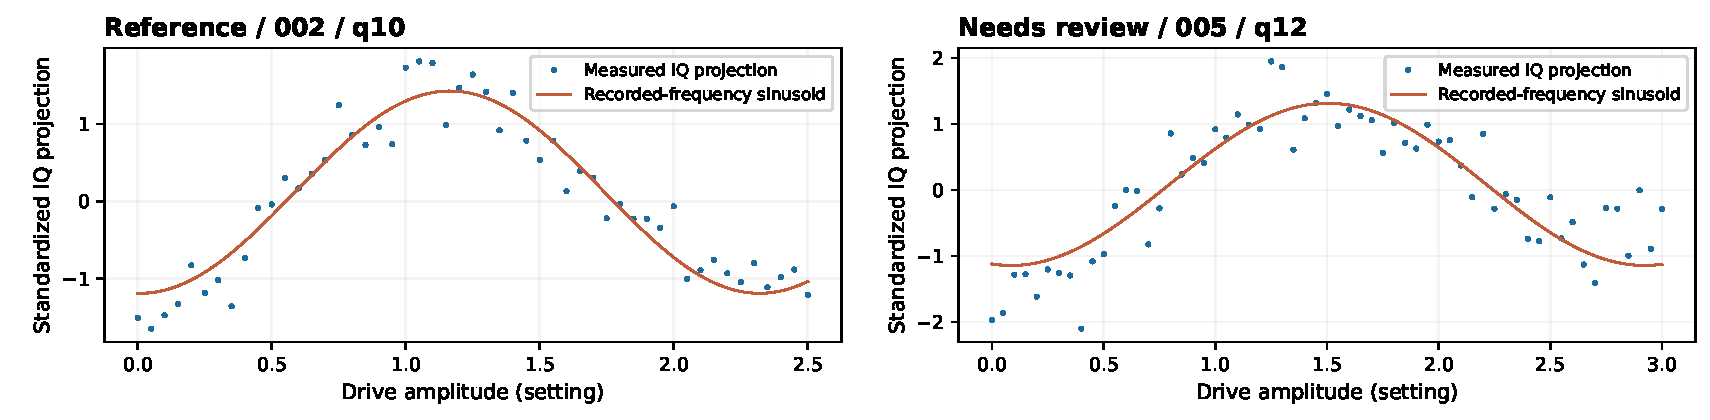
\includegraphics[width=\linewidth,height=34mm,keepaspectratio]{figures/rabi-005.pdf}
\caption{左：对照 002；右：案例 005。IQ 投影拟合： $R^2=0.798$；扫描覆盖 $1.06$ 个周期。IQ 投影独立标准化，符号与大小不可跨案例比较。}
\label{fig-rabi-005}
\end{figure}
\endgroup
{\small\textbf{判断：需检查完整 IQ 轨迹；投影与几何诊断尚不能确定物理原因。}\par}
\end{frame}

\begin{frame}[t,label=case-rabi-006]{IQ 分布偏离固定两态连线}{Rabi Oscillation / 006}
\setlength{\parskip}{0pt}
\begingroup
\setlength{\topsep}{0pt}\setlength{\partopsep}{0pt}
\begin{figure}
\centering
{\small
\makebox[.49\linewidth][c]{\textcolor{Teal}{左：转折与回返约束一个完整周期}}%
\makebox[.49\linewidth][c]{\textcolor{Orange}{右：投影拟合未验证两态连线近似}}\par
}
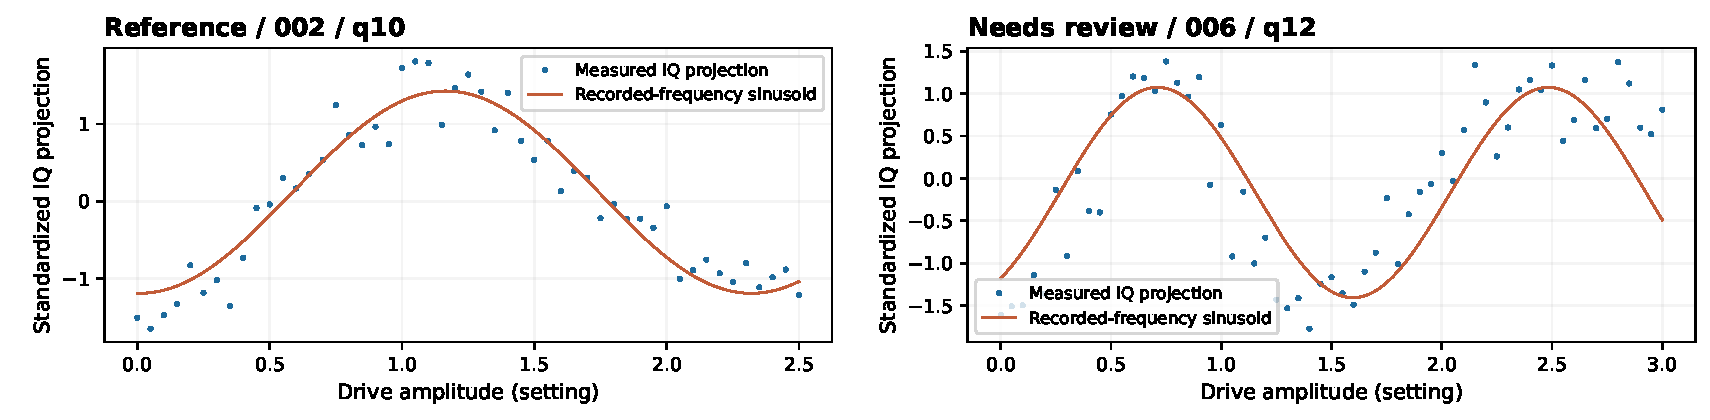
\includegraphics[width=\linewidth,height=34mm,keepaspectratio]{figures/rabi-006.pdf}
\caption{左：对照 002；右：案例 006。IQ 投影拟合： $R^2=0.689$；扫描覆盖 $1.69$ 个周期。IQ 投影独立标准化，符号与大小不可跨案例比较。}
\label{fig-rabi-006}
\end{figure}
\endgroup
{\small\textbf{判断：需检查完整 IQ 轨迹；投影与几何诊断尚不能确定物理原因。}\par}
\end{frame}

\begin{frame}[t,label=case-rabi-008]{局部曲线不足以约束周期}{Rabi Oscillation / 008}
\setlength{\parskip}{0pt}
\begingroup
\setlength{\topsep}{0pt}\setlength{\partopsep}{0pt}
\begin{figure}
\centering
{\small
\makebox[.49\linewidth][c]{\textcolor{Teal}{左：转折与回返约束一个完整周期}}%
\makebox[.49\linewidth][c]{\textcolor{Orange}{右：扫描只覆盖局部曲线}}\par
}
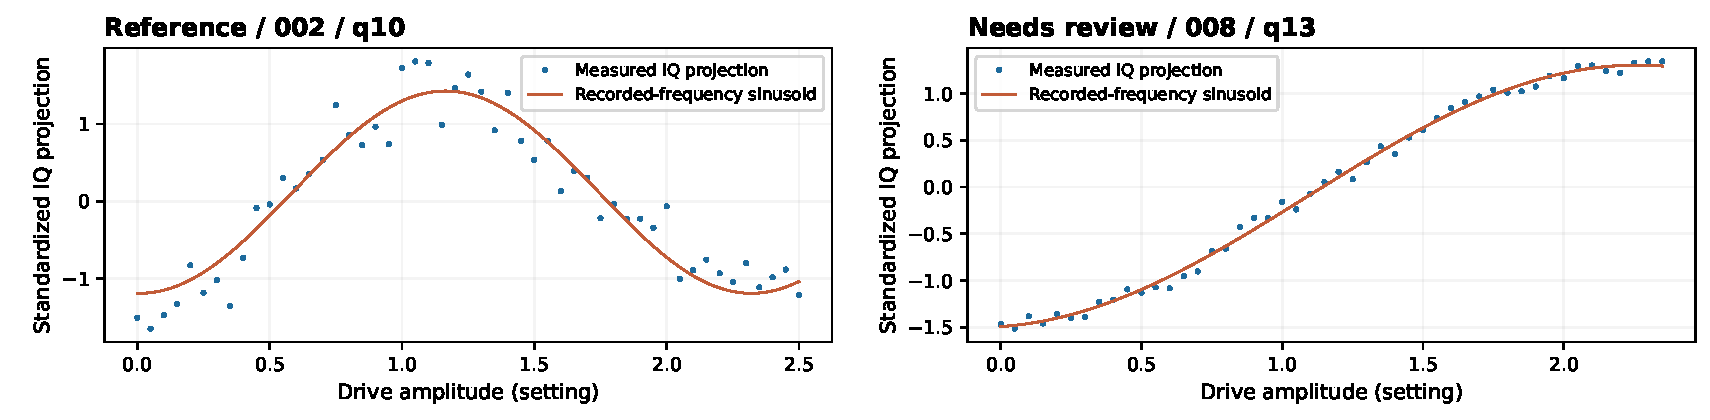
\includegraphics[width=\linewidth,height=34mm,keepaspectratio]{figures/rabi-008.pdf}
\caption{左：对照 002；右：案例 008。IQ 投影拟合： $R^2=0.996$；扫描覆盖 $0.50$ 个周期。IQ 投影独立标准化，符号与大小不可跨案例比较。}
\label{fig-rabi-008}
\end{figure}
\endgroup
{\small\textbf{判断：周期主要依赖外推；需扩大幅度范围，观察转折与回返。}\par}
\end{frame}

\begin{frame}[t,label=case-rabi-009]{单一正弦模型仍有未解释的结构}{Rabi Oscillation / 009}
\setlength{\parskip}{0pt}
\begingroup
\setlength{\topsep}{0pt}\setlength{\partopsep}{0pt}
\begin{figure}
\centering
{\small
\makebox[.49\linewidth][c]{\textcolor{Teal}{左：转折与回返约束一个完整周期}}%
\makebox[.49\linewidth][c]{\textcolor{Orange}{右：正弦拟合仍留下结构性残差}}\par
}
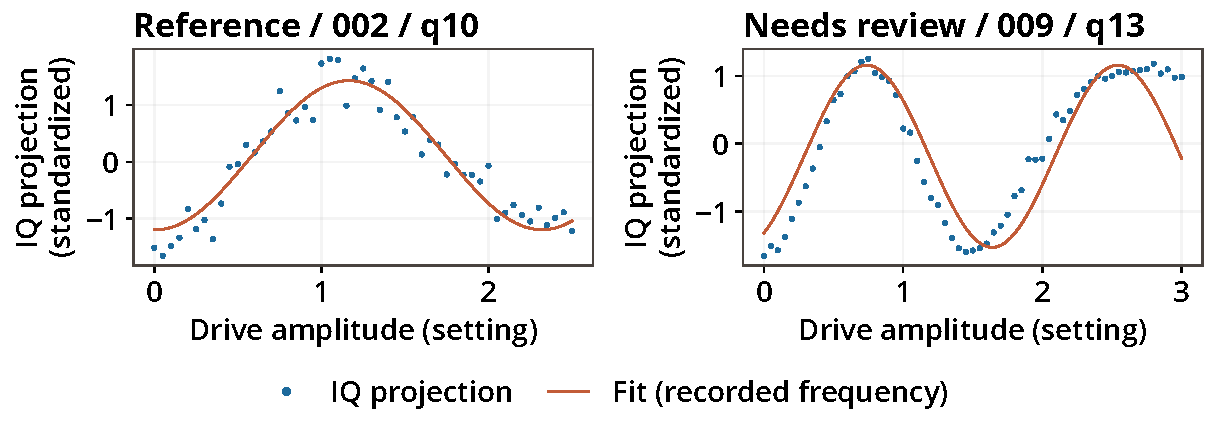
\includegraphics[width=\linewidth,height=34mm,keepaspectratio]{figures/rabi-009.pdf}
\caption{左：对照 002；右：案例 009。IQ 投影拟合： $R^2=0.824$；扫描覆盖 $1.66$ 个周期。IQ 投影独立标准化，符号与大小不可跨案例比较。}
\label{fig-rabi-009}
\end{figure}
\endgroup
{\small\textbf{判断：需复测并检查驱动与模型；单一正弦拟合尚不足以确认设置。}\par}
\end{frame}

\begin{frame}[t,label=case-rabi-010]{单一正弦模型仍有未解释的结构}{Rabi Oscillation / 010}
\setlength{\parskip}{0pt}
\begingroup
\setlength{\topsep}{0pt}\setlength{\partopsep}{0pt}
\begin{figure}
\centering
{\small
\makebox[.49\linewidth][c]{\textcolor{Teal}{左：转折与回返约束一个完整周期}}%
\makebox[.49\linewidth][c]{\textcolor{Orange}{右：正弦拟合仍留下结构性残差}}\par
}
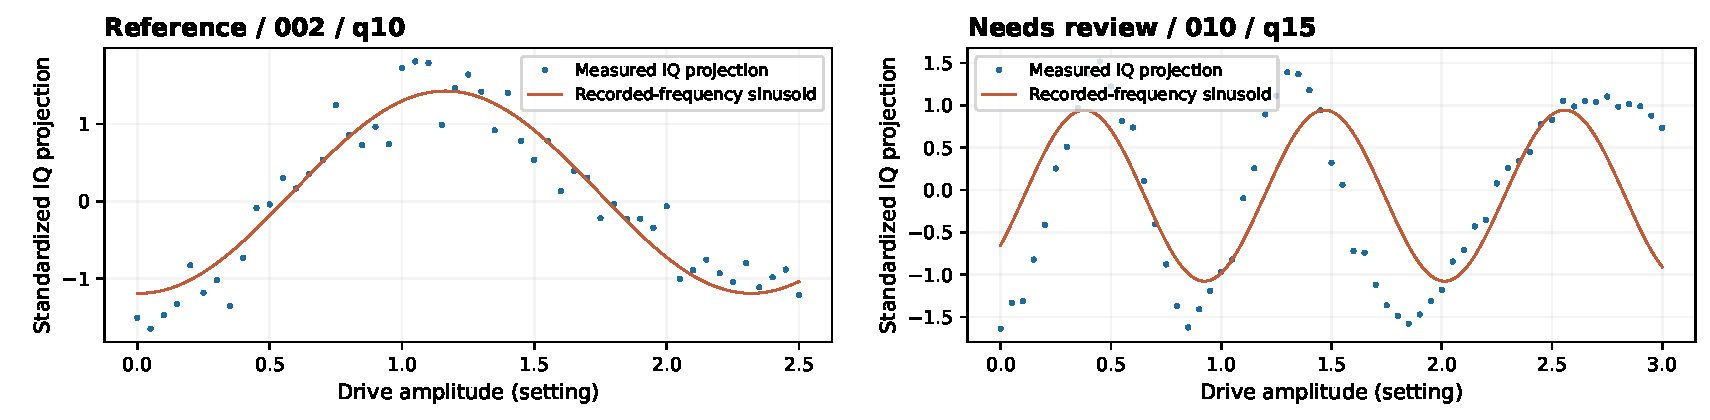
\includegraphics[width=\linewidth,height=34mm,keepaspectratio]{figures/rabi-010.pdf}
\caption{左：对照 002；右：案例 010。IQ 投影拟合： $R^2=0.480$；扫描覆盖 $2.76$ 个周期。IQ 投影独立标准化，符号与大小不可跨案例比较。}
\label{fig-rabi-010}
\end{figure}
\endgroup
{\small\textbf{判断：需复测并检查驱动与模型；单一正弦拟合尚不足以确认设置。}\par}
\end{frame}

\begin{frame}[t,label=case-rabi-011]{单一正弦模型仍有未解释的结构}{Rabi Oscillation / 011}
\setlength{\parskip}{0pt}
\begingroup
\setlength{\topsep}{0pt}\setlength{\partopsep}{0pt}
\begin{figure}
\centering
{\small
\makebox[.49\linewidth][c]{\textcolor{Teal}{左：转折与回返约束一个完整周期}}%
\makebox[.49\linewidth][c]{\textcolor{Orange}{右：正弦拟合仍留下结构性残差}}\par
}
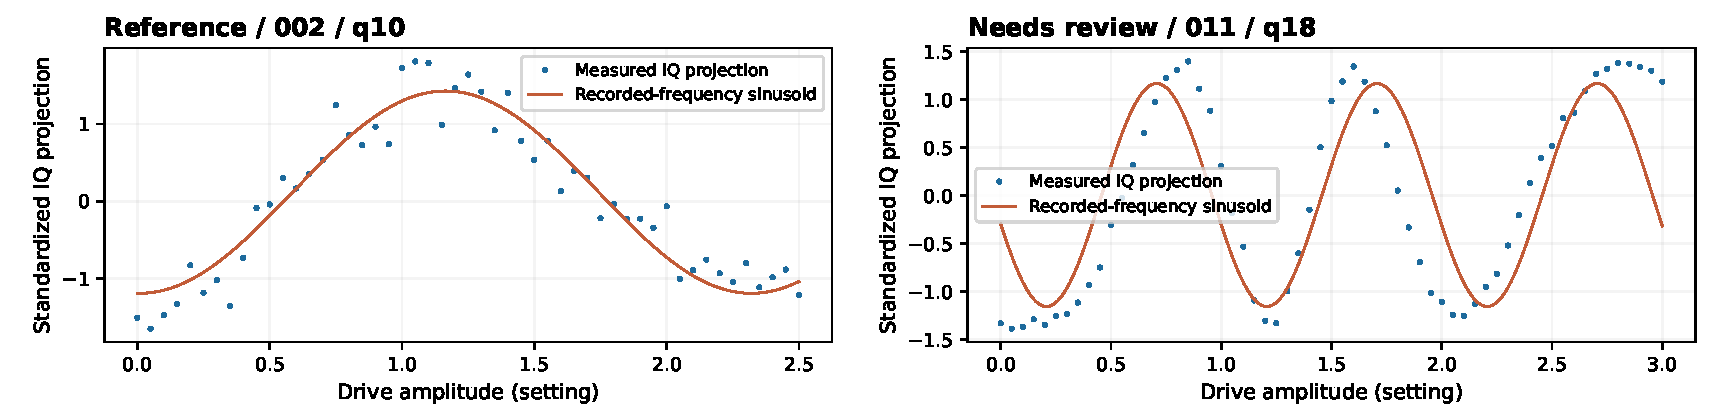
\includegraphics[width=\linewidth,height=34mm,keepaspectratio]{figures/rabi-011.pdf}
\caption{左：对照 002；右：案例 011。IQ 投影拟合： $R^2=0.664$；扫描覆盖 $3.00$ 个周期。IQ 投影独立标准化，符号与大小不可跨案例比较。}
\label{fig-rabi-011}
\end{figure}
\endgroup
{\small\textbf{判断：需复测并检查驱动与模型；单一正弦拟合尚不足以确认设置。}\par}
\end{frame}

\begin{frame}[t,label=case-rabi-012]{单一正弦模型仍有未解释的结构}{Rabi Oscillation / 012}
\setlength{\parskip}{0pt}
\begingroup
\setlength{\topsep}{0pt}\setlength{\partopsep}{0pt}
\begin{figure}
\centering
{\small
\makebox[.49\linewidth][c]{\textcolor{Teal}{左：转折与回返约束一个完整周期}}%
\makebox[.49\linewidth][c]{\textcolor{Orange}{右：正弦拟合仍留下结构性残差}}\par
}
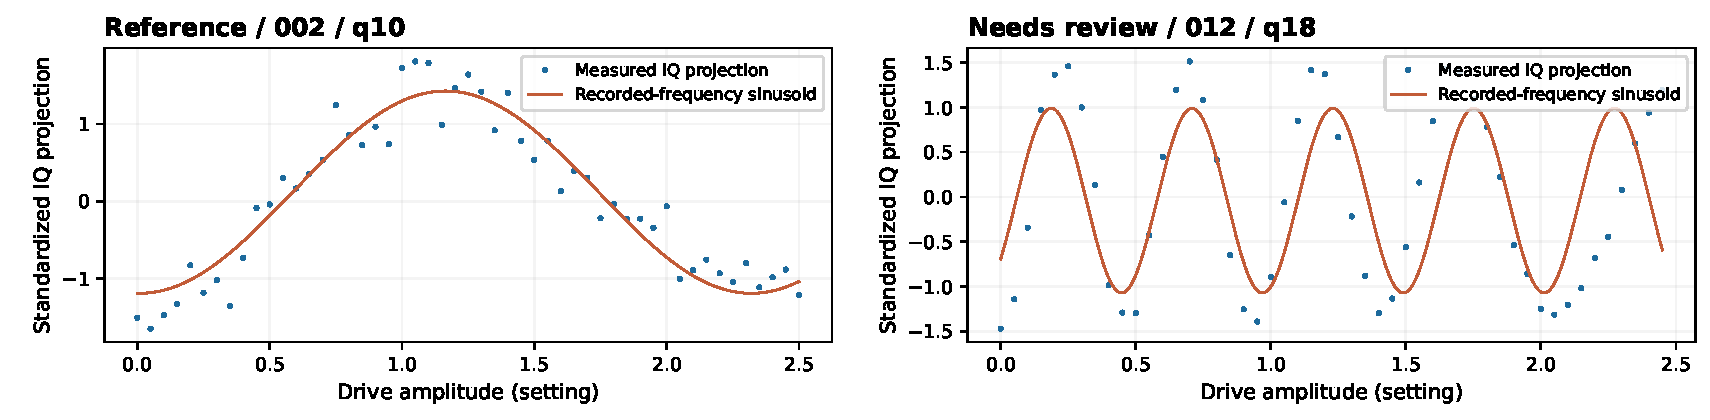
\includegraphics[width=\linewidth,height=34mm,keepaspectratio]{figures/rabi-012.pdf}
\caption{左：对照 002；右：案例 012。IQ 投影拟合： $R^2=0.512$；扫描覆盖 $4.70$ 个周期。IQ 投影独立标准化，符号与大小不可跨案例比较。}
\label{fig-rabi-012}
\end{figure}
\endgroup
{\small\textbf{判断：需复测并检查驱动与模型；单一正弦拟合尚不足以确认设置。}\par}
\end{frame}

\begin{frame}[t,label=case-rabi-013]{单一正弦模型仍有未解释的结构}{Rabi Oscillation / 013}
\setlength{\parskip}{0pt}
\begingroup
\setlength{\topsep}{0pt}\setlength{\partopsep}{0pt}
\begin{figure}
\centering
{\small
\makebox[.49\linewidth][c]{\textcolor{Teal}{左：转折与回返约束一个完整周期}}%
\makebox[.49\linewidth][c]{\textcolor{Orange}{右：正弦拟合仍留下结构性残差}}\par
}
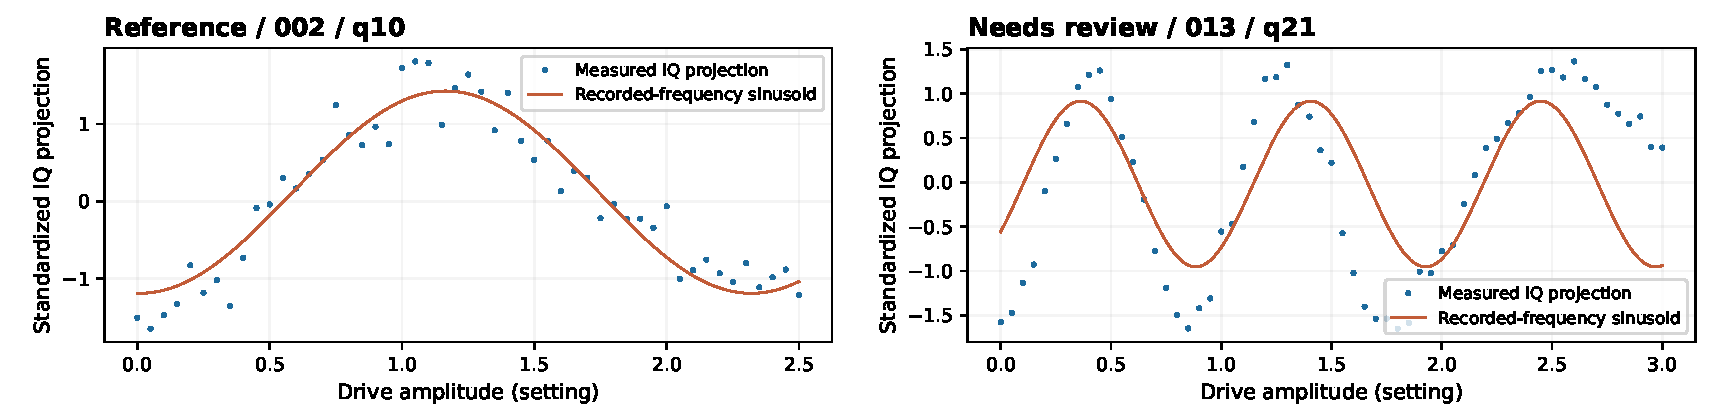
\includegraphics[width=\linewidth,height=34mm,keepaspectratio]{figures/rabi-013.pdf}
\caption{左：对照 002；右：案例 013。IQ 投影拟合： $R^2=0.432$；扫描覆盖 $2.88$ 个周期。IQ 投影独立标准化，符号与大小不可跨案例比较。}
\label{fig-rabi-013}
\end{figure}
\endgroup
{\small\textbf{判断：需复测并检查驱动与模型；单一正弦拟合尚不足以确认设置。}\par}
\end{frame}

\begin{frame}[t,label=case-rabi-014]{单一正弦模型仍有未解释的结构}{Rabi Oscillation / 014}
\setlength{\parskip}{0pt}
\begingroup
\setlength{\topsep}{0pt}\setlength{\partopsep}{0pt}
\begin{figure}
\centering
{\small
\makebox[.49\linewidth][c]{\textcolor{Teal}{左：转折与回返约束一个完整周期}}%
\makebox[.49\linewidth][c]{\textcolor{Orange}{右：正弦拟合仍留下结构性残差}}\par
}
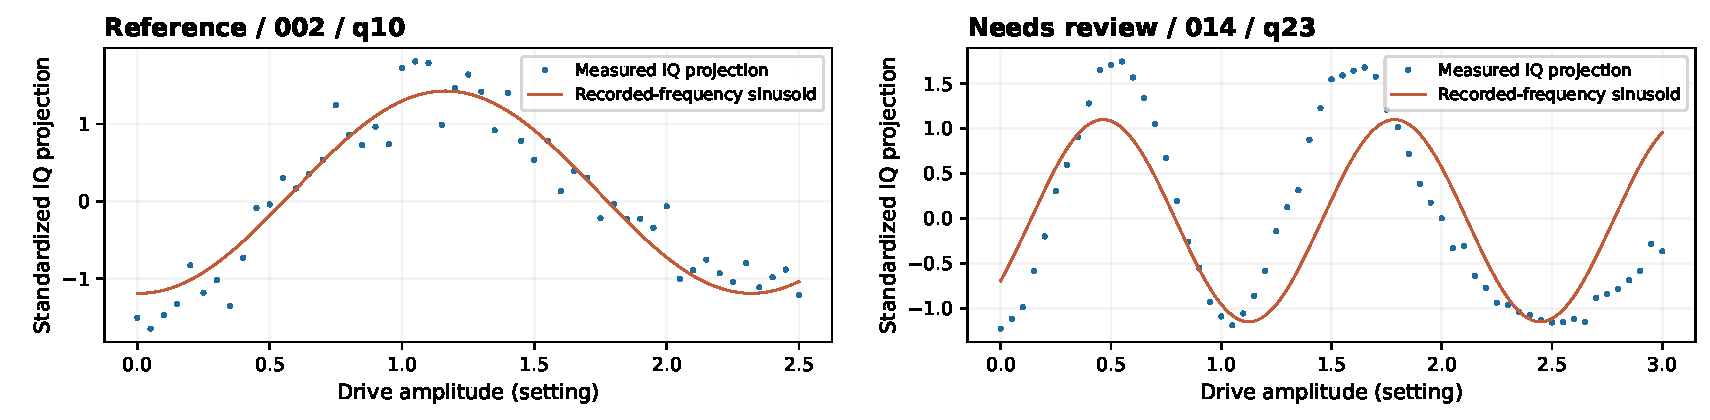
\includegraphics[width=\linewidth,height=34mm,keepaspectratio]{figures/rabi-014.pdf}
\caption{左：对照 002；右：案例 014。IQ 投影拟合： $R^2=0.594$；扫描覆盖 $2.27$ 个周期。IQ 投影独立标准化，符号与大小不可跨案例比较。}
\label{fig-rabi-014}
\end{figure}
\endgroup
{\small\textbf{判断：需复测并检查驱动与模型；单一正弦拟合尚不足以确认设置。}\par}
\end{frame}

\begin{frame}[t,label=case-rabi-015]{局部曲线不足以约束周期}{Rabi Oscillation / 015}
\setlength{\parskip}{0pt}
\begingroup
\setlength{\topsep}{0pt}\setlength{\partopsep}{0pt}
\begin{figure}
\centering
{\small
\makebox[.49\linewidth][c]{\textcolor{Teal}{左：转折与回返约束一个完整周期}}%
\makebox[.49\linewidth][c]{\textcolor{Orange}{右：扫描只覆盖局部曲线}}\par
}
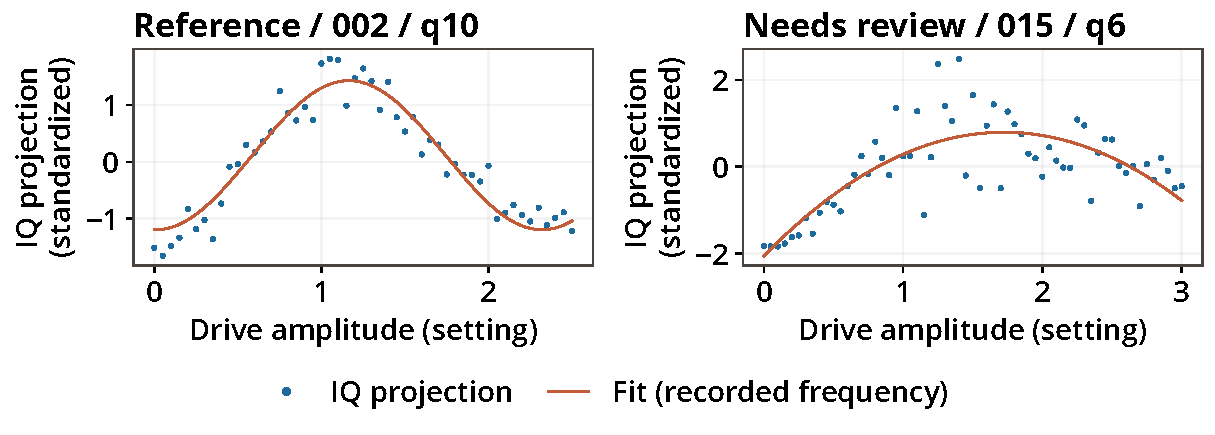
\includegraphics[width=\linewidth,height=34mm,keepaspectratio]{figures/rabi-015.pdf}
\caption{左：对照 002；右：案例 015。IQ 投影拟合： $R^2=0.586$；扫描覆盖 $0.10$ 个周期。IQ 投影独立标准化，符号与大小不可跨案例比较。}
\label{fig-rabi-015}
\end{figure}
\endgroup
{\small\textbf{判断：周期主要依赖外推；需扩大幅度范围，观察转折与回返。}\par}
\end{frame}

\begin{frame}[t,label=case-rabi-016]{单一正弦模型仍有未解释的结构}{Rabi Oscillation / 016}
\setlength{\parskip}{0pt}
\begingroup
\setlength{\topsep}{0pt}\setlength{\partopsep}{0pt}
\begin{figure}
\centering
{\small
\makebox[.49\linewidth][c]{\textcolor{Teal}{左：转折与回返约束一个完整周期}}%
\makebox[.49\linewidth][c]{\textcolor{Orange}{右：正弦拟合仍留下结构性残差}}\par
}
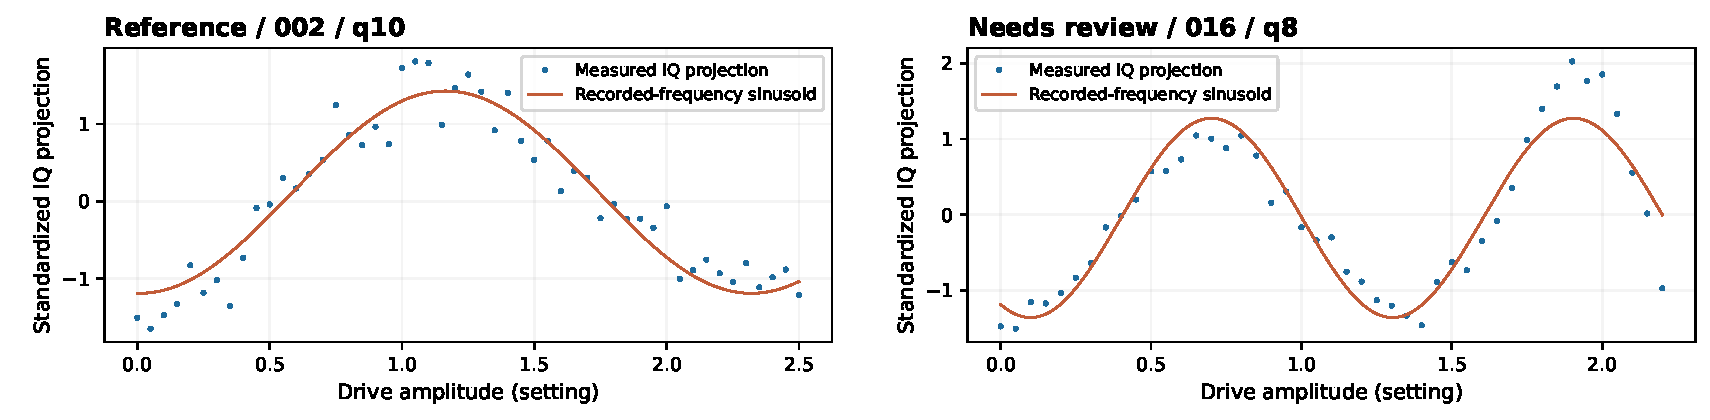
\includegraphics[width=\linewidth,height=34mm,keepaspectratio]{figures/rabi-016.pdf}
\caption{左：对照 002；右：案例 016。IQ 投影拟合： $R^2=0.894$；扫描覆盖 $1.83$ 个周期。IQ 投影独立标准化，符号与大小不可跨案例比较。}
\label{fig-rabi-016}
\end{figure}
\endgroup
{\small\textbf{判断：需复测并检查驱动与模型；单一正弦拟合尚不足以确认设置。}\par}
\end{frame}

\begin{frame}[t,label=case-spectroscopy-002]{背景中的候选响应仍需验证}{Qubit Spectroscopy / 002}
\setlength{\parskip}{0pt}
\begingroup
\setlength{\topsep}{0pt}\setlength{\partopsep}{0pt}
\begin{figure}
\centering
{\small
\makebox[.49\linewidth][c]{\textcolor{Teal}{左：窗口内可见响应与两侧背景}}%
\makebox[.49\linewidth][c]{\textcolor{Orange}{右：背景中的候选响应不够明确}}\par
}
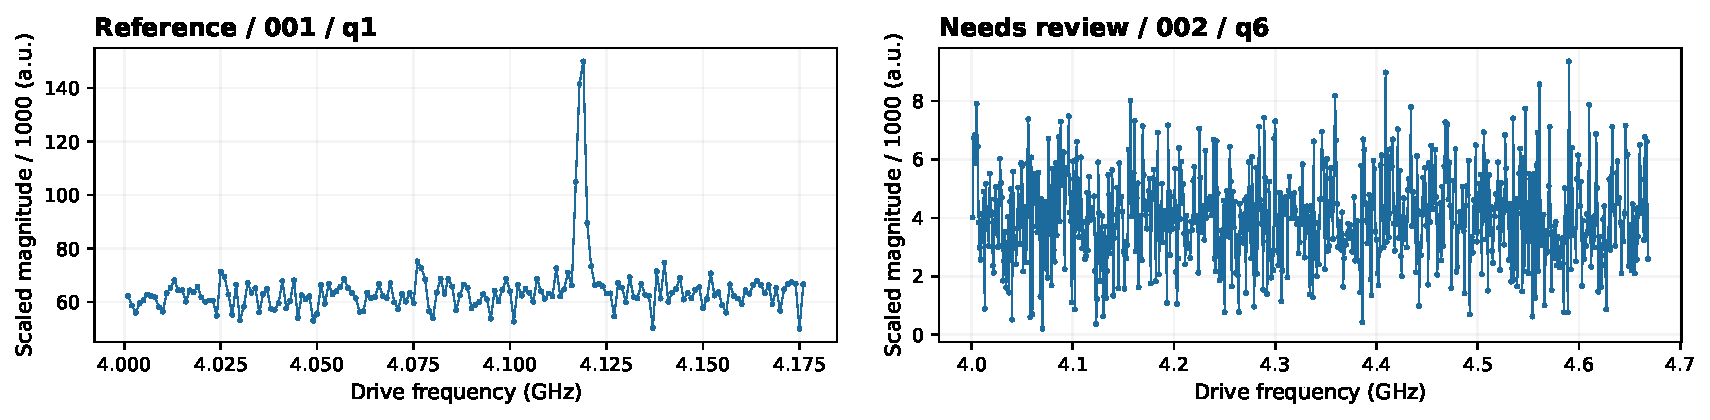
\includegraphics[width=\linewidth,height=34mm,keepaspectratio]{figures/spectroscopy-002.pdf}
\caption{左：对照 001；右：案例 002。IQ 投影诊断： $R^2=0.016$；步长 1.00 / 半高全宽 1.08 MHz。图示幅度；指标来自 IQ 投影的单洛伦兹线形拟合。}
\label{fig-spectroscopy-002}
\end{figure}
\endgroup
{\small\textbf{判断：尚不能确认跃迁频率；需验证信号路径并复测候选响应。}\par}
\end{frame}

\begin{frame}[t,label=case-spectroscopy-004]{可见响应仍需检查线形模型}{Qubit Spectroscopy / 004}
\setlength{\parskip}{0pt}
\begingroup
\setlength{\topsep}{0pt}\setlength{\partopsep}{0pt}
\begin{figure}
\centering
{\small
\makebox[.49\linewidth][c]{\textcolor{Teal}{左：窗口内可见响应与两侧背景}}%
\makebox[.49\linewidth][c]{\textcolor{Orange}{右：单线形拟合仍有未解释结构}}\par
}
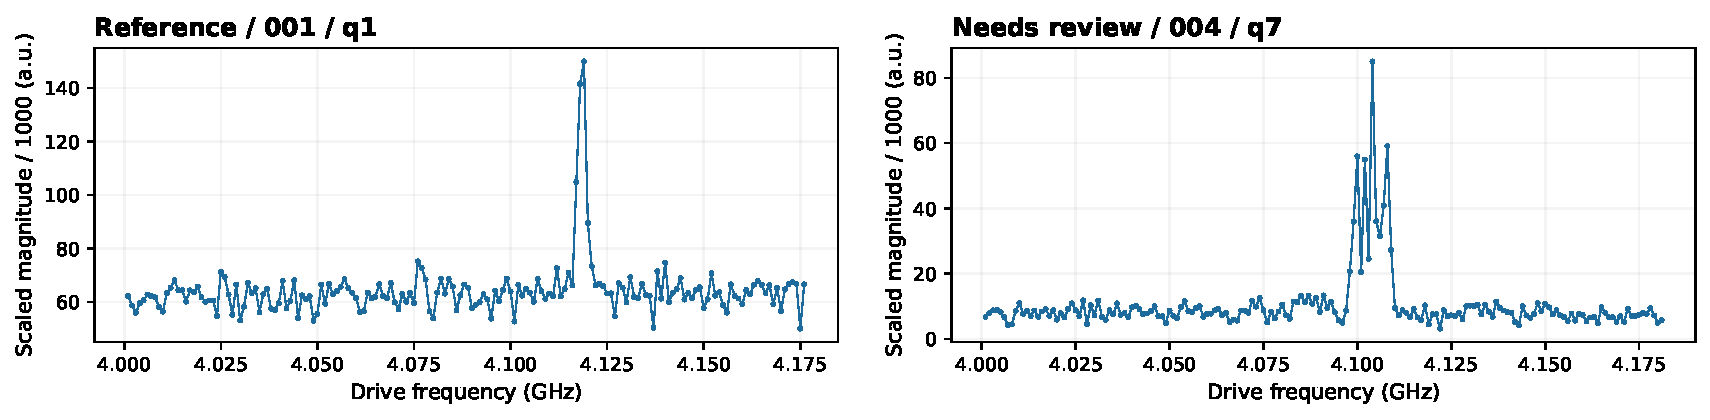
\includegraphics[width=\linewidth,height=34mm,keepaspectratio]{figures/spectroscopy-004.pdf}
\caption{左：对照 001；右：案例 004。IQ 投影诊断： $R^2=0.682$；步长 1.00 / 半高全宽 7.55 MHz。图示幅度；指标来自 IQ 投影的单洛伦兹线形拟合。}
\label{fig-spectroscopy-004}
\end{figure}
\endgroup
{\small\textbf{判断：可见响应不保证单线形模型适用；需细扫并检查线形与背景。}\par}
\end{frame}

\begin{frame}[t,label=case-spectroscopy-006]{可见响应仍需检查线形模型}{Qubit Spectroscopy / 006}
\setlength{\parskip}{0pt}
\begingroup
\setlength{\topsep}{0pt}\setlength{\partopsep}{0pt}
\begin{figure}
\centering
{\small
\makebox[.49\linewidth][c]{\textcolor{Teal}{左：窗口内可见响应与两侧背景}}%
\makebox[.49\linewidth][c]{\textcolor{Orange}{右：单线形拟合仍有未解释结构}}\par
}
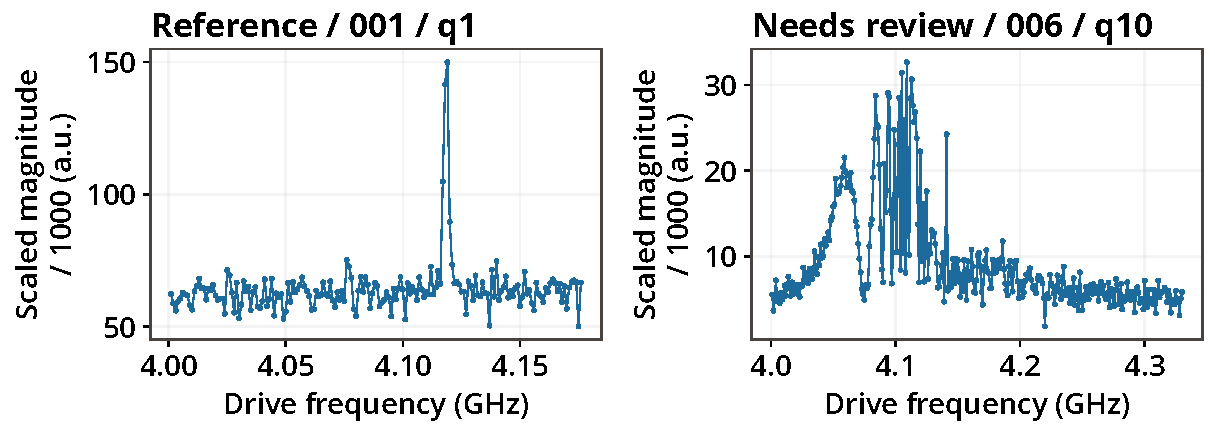
\includegraphics[width=\linewidth,height=34mm,keepaspectratio]{figures/spectroscopy-006.pdf}
\caption{左：对照 001；右：案例 006。IQ 投影诊断： $R^2=0.545$；步长 1.00 / 半高全宽 116.37 MHz。图示幅度；指标来自 IQ 投影的单洛伦兹线形拟合。}
\label{fig-spectroscopy-006}
\end{figure}
\endgroup
{\small\textbf{判断：可见响应不保证单线形模型适用；需细扫并检查线形与背景。}\par}
\end{frame}

\begin{frame}[t,label=case-spectroscopy-007]{频率步长不能分辨拟合线宽}{Qubit Spectroscopy / 007}
\setlength{\parskip}{0pt}
\begingroup
\setlength{\topsep}{0pt}\setlength{\partopsep}{0pt}
\begin{figure}
\centering
{\small
\makebox[.49\linewidth][c]{\textcolor{Teal}{左：窗口内可见响应与两侧背景}}%
\makebox[.49\linewidth][c]{\textcolor{Orange}{右：候选线宽内采样点不足}}\par
}
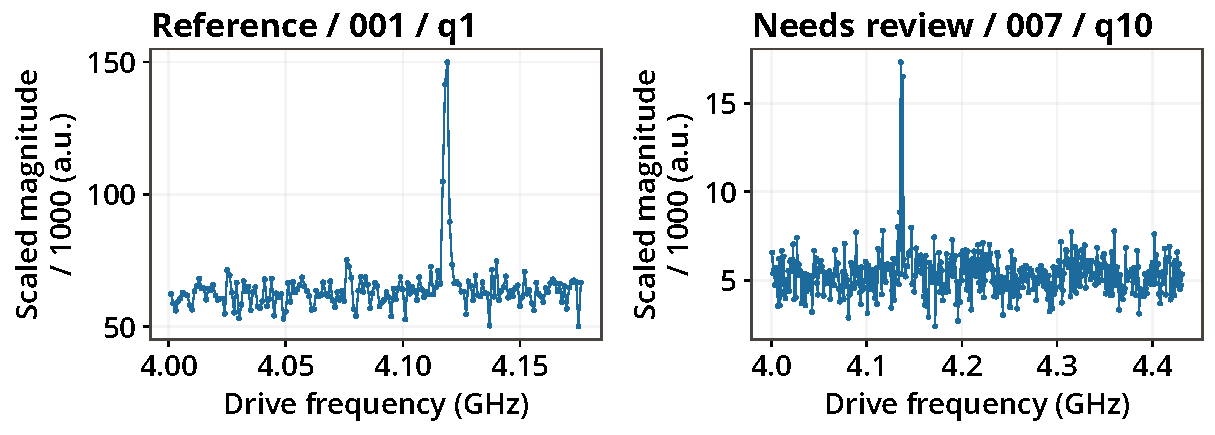
\includegraphics[width=\linewidth,height=34mm,keepaspectratio]{figures/spectroscopy-007.pdf}
\caption{左：对照 001；右：案例 007。IQ 投影诊断： $R^2=0.265$；步长 1.00 / 半高全宽 1.57 MHz。图示幅度；指标来自 IQ 投影的单洛伦兹线形拟合。}
\label{fig-spectroscopy-007}
\end{figure}
\endgroup
{\small\textbf{判断：线宽缺乏采样约束；需局部细扫并复测。}\par}
\end{frame}

\begin{frame}[t,label=case-spectroscopy-009]{频率步长不能分辨拟合线宽}{Qubit Spectroscopy / 009}
\setlength{\parskip}{0pt}
\begingroup
\setlength{\topsep}{0pt}\setlength{\partopsep}{0pt}
\begin{figure}
\centering
{\small
\makebox[.49\linewidth][c]{\textcolor{Teal}{左：窗口内可见响应与两侧背景}}%
\makebox[.49\linewidth][c]{\textcolor{Orange}{右：候选线宽内采样点不足}}\par
}
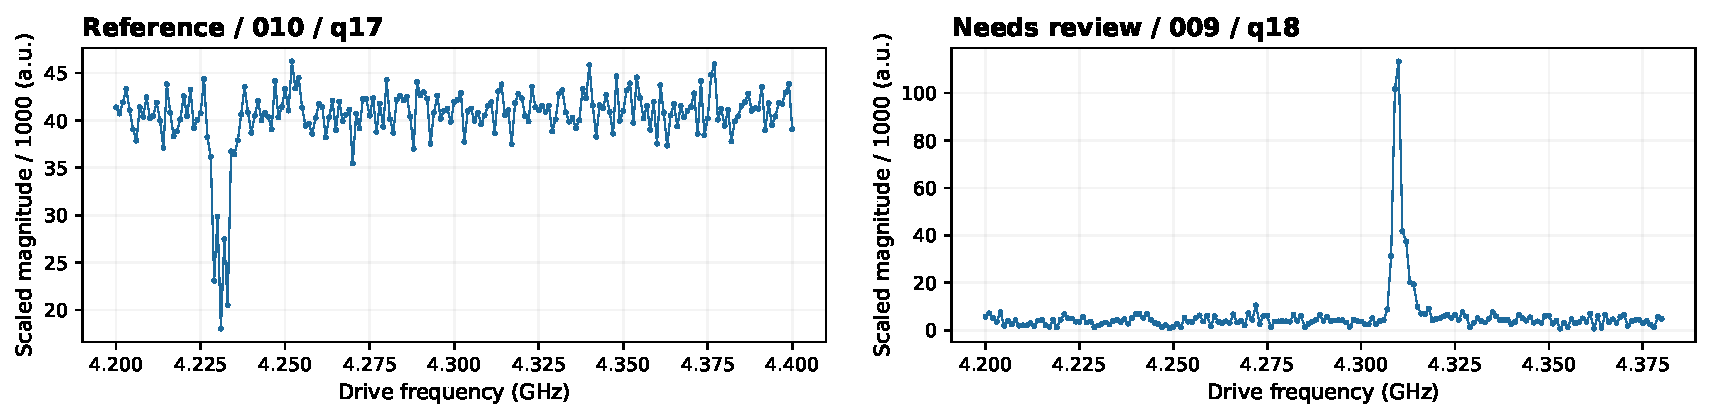
\includegraphics[width=\linewidth,height=34mm,keepaspectratio]{figures/spectroscopy-009.pdf}
\caption{左：对照 010；右：案例 009。IQ 投影诊断： $R^2=0.948$；步长 1.00 / 半高全宽 1.85 MHz。图示幅度；指标来自 IQ 投影的单洛伦兹线形拟合。}
\label{fig-spectroscopy-009}
\end{figure}
\endgroup
{\small\textbf{判断：线宽缺乏采样约束；需局部细扫并复测。}\par}
\end{frame}

\begin{frame}[t,label=case-spectroscopy-011]{背景中的候选响应仍需验证}{Qubit Spectroscopy / 011}
\setlength{\parskip}{0pt}
\begingroup
\setlength{\topsep}{0pt}\setlength{\partopsep}{0pt}
\begin{figure}
\centering
{\small
\makebox[.49\linewidth][c]{\textcolor{Teal}{左：窗口内可见响应与两侧背景}}%
\makebox[.49\linewidth][c]{\textcolor{Orange}{右：背景中的候选响应不够明确}}\par
}
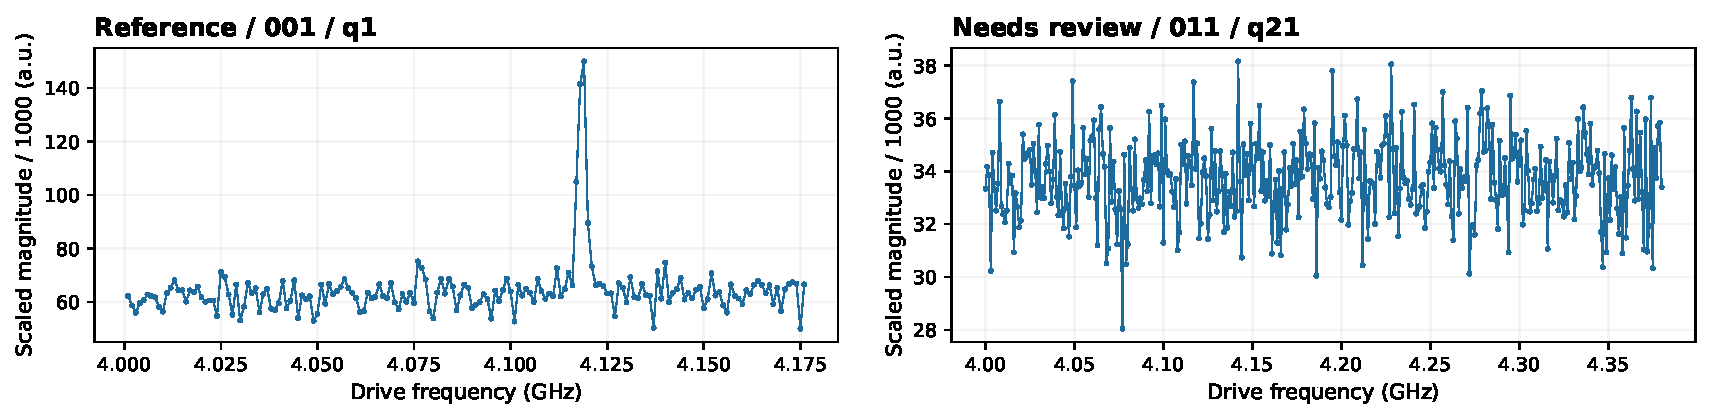
\includegraphics[width=\linewidth,height=34mm,keepaspectratio]{figures/spectroscopy-011.pdf}
\caption{左：对照 001；右：案例 011。IQ 投影诊断： $R^2=0.044$；步长 1.00 / 半高全宽 2.11 MHz。图示幅度；指标来自 IQ 投影的单洛伦兹线形拟合。}
\label{fig-spectroscopy-011}
\end{figure}
\endgroup
{\small\textbf{判断：尚不能确认跃迁频率；需验证信号路径并复测候选响应。}\par}
\end{frame}

\begin{frame}[t,label=case-spectroscopy-012]{扫描边界限制了中心频率的判断}{Qubit Spectroscopy / 012}
\setlength{\parskip}{0pt}
\begingroup
\setlength{\topsep}{0pt}\setlength{\partopsep}{0pt}
\begin{figure}
\centering
{\small
\makebox[.49\linewidth][c]{\textcolor{Teal}{左：窗口内可见响应与两侧背景}}%
\makebox[.49\linewidth][c]{\textcolor{Orange}{右：边缘响应未被完整覆盖}}\par
}
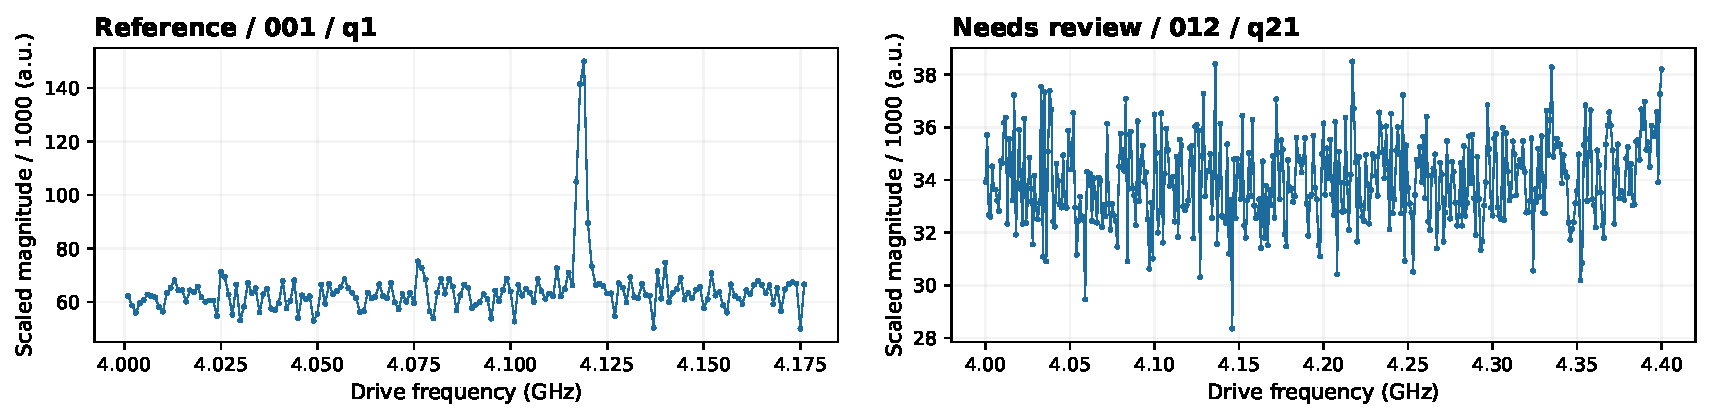
\includegraphics[width=\linewidth,height=34mm,keepaspectratio]{figures/spectroscopy-012.pdf}
\caption{左：对照 001；右：案例 012。IQ 投影诊断： $R^2=0.065$；步长 1.00 / 半高全宽 782.41 MHz。图示幅度；指标来自 IQ 投影的单洛伦兹线形拟合。}
\label{fig-spectroscopy-012}
\end{figure}
\endgroup
{\small\textbf{判断：中心频率缺乏两侧数据约束；需扩大扫描窗口。}\par}
\end{frame}

\begin{frame}[t,label=case-spectroscopy-013]{可见响应仍需检查线形模型}{Qubit Spectroscopy / 013}
\setlength{\parskip}{0pt}
\begingroup
\setlength{\topsep}{0pt}\setlength{\partopsep}{0pt}
\begin{figure}
\centering
{\small
\makebox[.49\linewidth][c]{\textcolor{Teal}{左：窗口内可见响应与两侧背景}}%
\makebox[.49\linewidth][c]{\textcolor{Orange}{右：单线形拟合仍有未解释结构}}\par
}
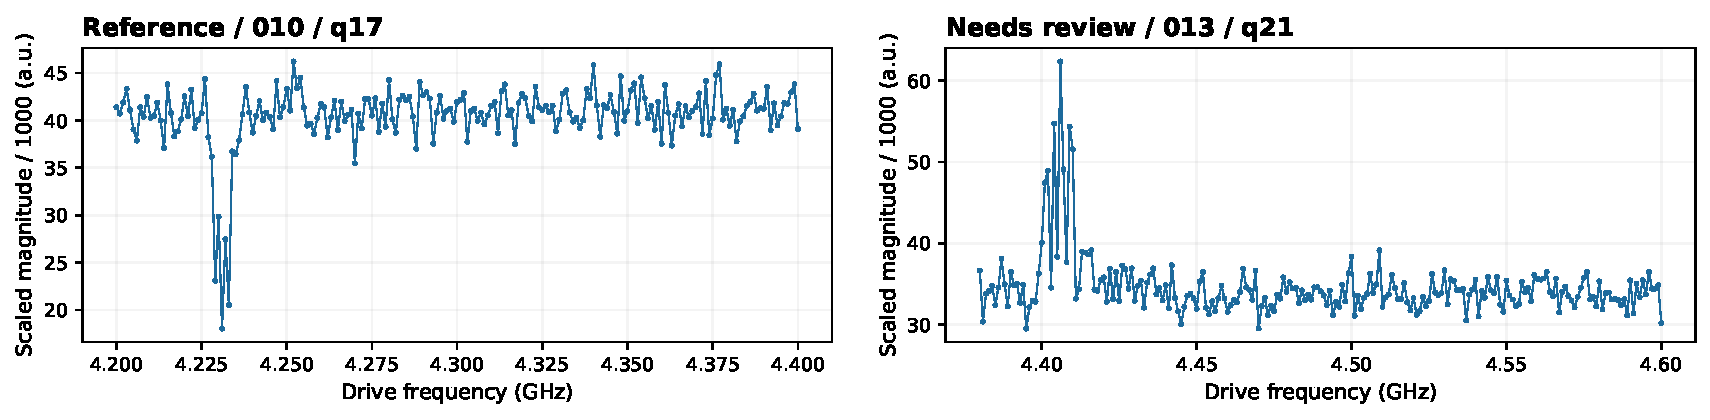
\includegraphics[width=\linewidth,height=34mm,keepaspectratio]{figures/spectroscopy-013.pdf}
\caption{左：对照 010；右：案例 013。IQ 投影诊断： $R^2=0.618$；步长 1.00 / 半高全宽 8.93 MHz。图示幅度；指标来自 IQ 投影的单洛伦兹线形拟合。}
\label{fig-spectroscopy-013}
\end{figure}
\endgroup
{\small\textbf{判断：可见响应不保证单线形模型适用；需细扫并检查线形与背景。}\par}
\end{frame}

\begin{frame}[t,label=case-spectroscopy-014]{背景中的候选响应仍需验证}{Qubit Spectroscopy / 014}
\setlength{\parskip}{0pt}
\begingroup
\setlength{\topsep}{0pt}\setlength{\partopsep}{0pt}
\begin{figure}
\centering
{\small
\makebox[.49\linewidth][c]{\textcolor{Teal}{左：窗口内可见响应与两侧背景}}%
\makebox[.49\linewidth][c]{\textcolor{Orange}{右：背景中的候选响应不够明确}}\par
}
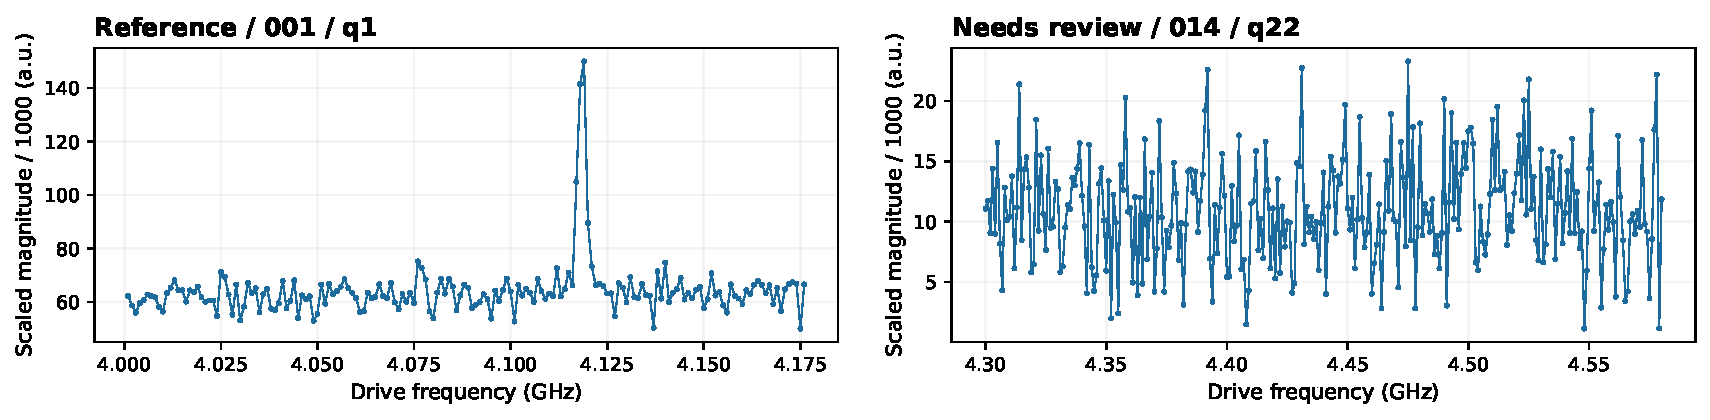
\includegraphics[width=\linewidth,height=34mm,keepaspectratio]{figures/spectroscopy-014.pdf}
\caption{左：对照 001；右：案例 014。IQ 投影诊断： $R^2=0.033$；步长 1.00 / 半高全宽 1.01 MHz。图示幅度；指标来自 IQ 投影的单洛伦兹线形拟合。}
\label{fig-spectroscopy-014}
\end{figure}
\endgroup
{\small\textbf{判断：尚不能确认跃迁频率；需验证信号路径并复测候选响应。}\par}
\end{frame}

\begin{frame}[t,label=case-spectroscopy-015]{背景中的候选响应仍需验证}{Qubit Spectroscopy / 015}
\setlength{\parskip}{0pt}
\begingroup
\setlength{\topsep}{0pt}\setlength{\partopsep}{0pt}
\begin{figure}
\centering
{\small
\makebox[.49\linewidth][c]{\textcolor{Teal}{左：窗口内可见响应与两侧背景}}%
\makebox[.49\linewidth][c]{\textcolor{Orange}{右：背景中的候选响应不够明确}}\par
}
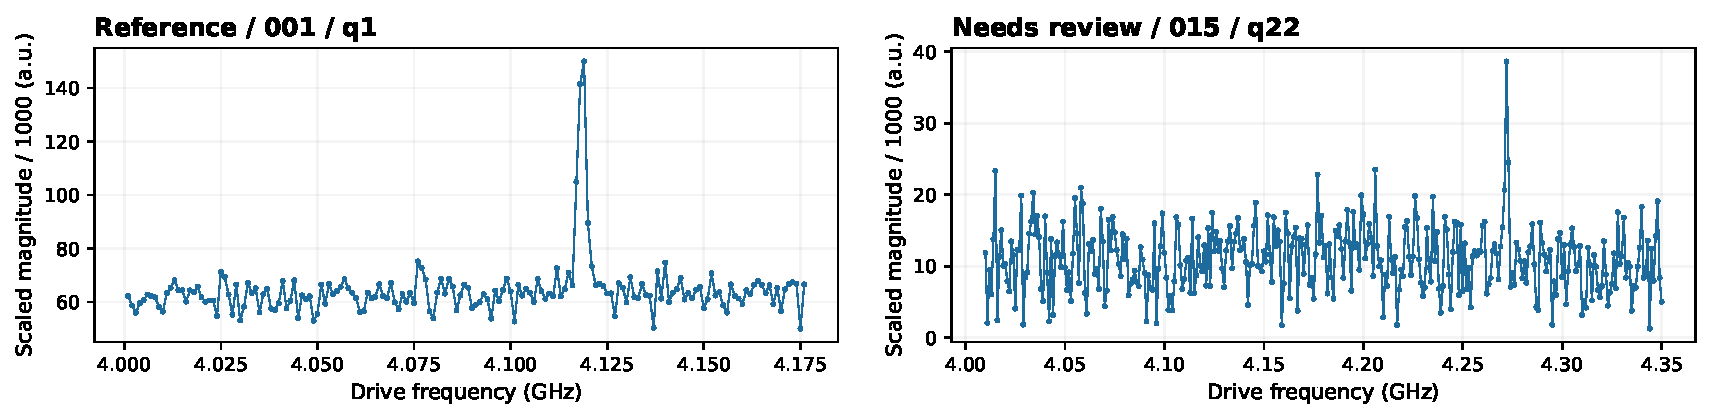
\includegraphics[width=\linewidth,height=34mm,keepaspectratio]{figures/spectroscopy-015.pdf}
\caption{左：对照 001；右：案例 015。IQ 投影诊断： $R^2=0.054$；步长 1.00 / 半高全宽 2.01 MHz。图示幅度；指标来自 IQ 投影的单洛伦兹线形拟合。}
\label{fig-spectroscopy-015}
\end{figure}
\endgroup
{\small\textbf{判断：尚不能确认跃迁频率；需验证信号路径并复测候选响应。}\par}
\end{frame}

\begin{frame}[t,label=case-spectroscopy-016]{可见响应仍需检查线形模型}{Qubit Spectroscopy / 016}
\setlength{\parskip}{0pt}
\begingroup
\setlength{\topsep}{0pt}\setlength{\partopsep}{0pt}
\begin{figure}
\centering
{\small
\makebox[.49\linewidth][c]{\textcolor{Teal}{左：窗口内可见响应与两侧背景}}%
\makebox[.49\linewidth][c]{\textcolor{Orange}{右：单线形拟合仍有未解释结构}}\par
}
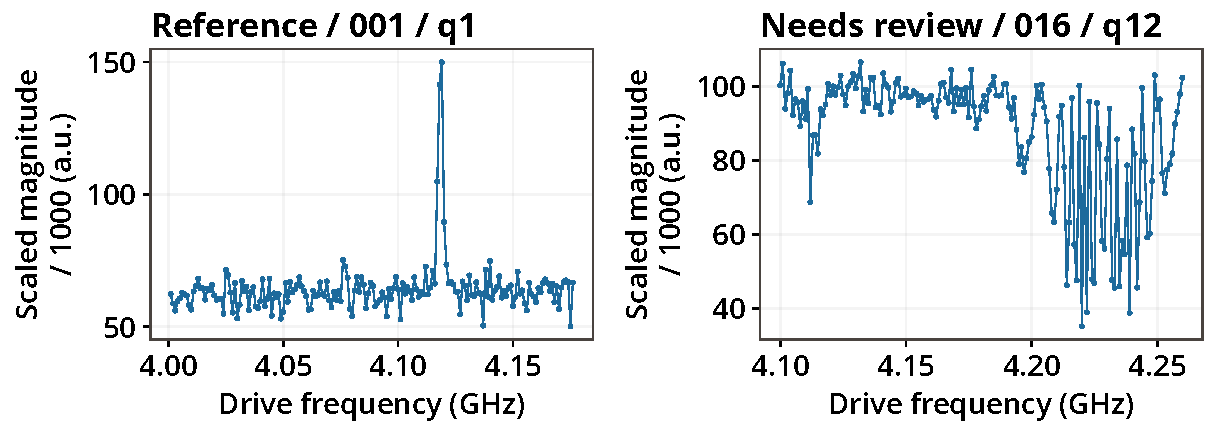
\includegraphics[width=\linewidth,height=34mm,keepaspectratio]{figures/spectroscopy-016.pdf}
\caption{左：对照 001；右：案例 016。IQ 投影诊断： $R^2=0.392$；步长 1.00 / 半高全宽 54.00 MHz。图示幅度；指标来自 IQ 投影的单洛伦兹线形拟合。}
\label{fig-spectroscopy-016}
\end{figure}
\endgroup
{\small\textbf{判断：可见响应不保证单线形模型适用；需细扫并检查线形与背景。}\par}
\end{frame}

\begin{frame}[t,label=case-spectroscopy-017]{可见响应仍需检查线形模型}{Qubit Spectroscopy / 017}
\setlength{\parskip}{0pt}
\begingroup
\setlength{\topsep}{0pt}\setlength{\partopsep}{0pt}
\begin{figure}
\centering
{\small
\makebox[.49\linewidth][c]{\textcolor{Teal}{左：窗口内可见响应与两侧背景}}%
\makebox[.49\linewidth][c]{\textcolor{Orange}{右：单线形拟合仍有未解释结构}}\par
}
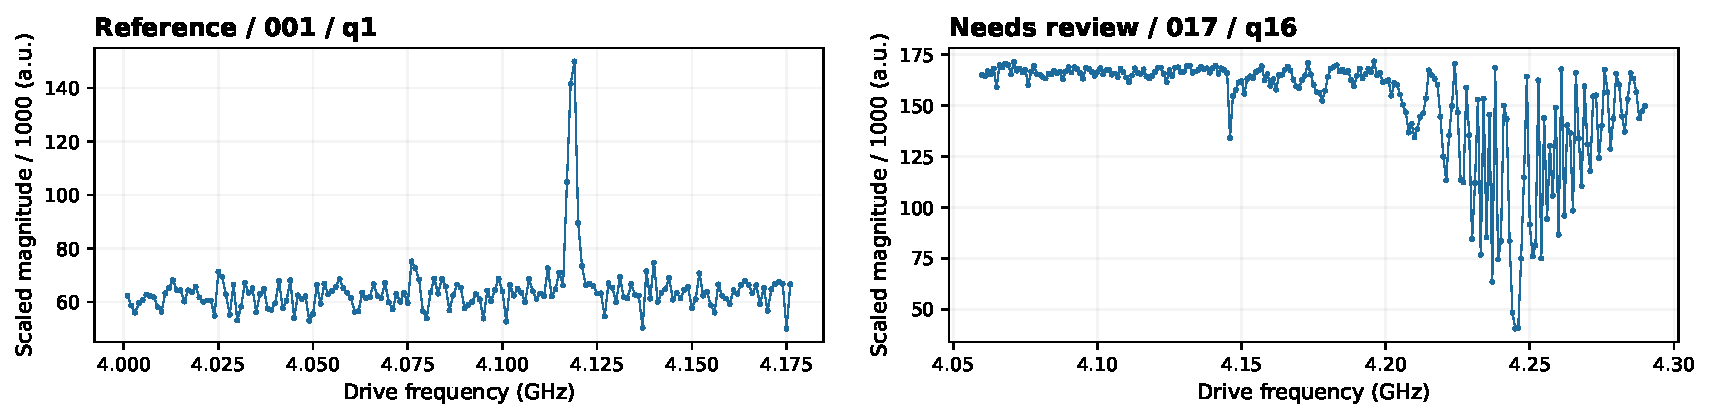
\includegraphics[width=\linewidth,height=34mm,keepaspectratio]{figures/spectroscopy-017.pdf}
\caption{左：对照 001；右：案例 017。IQ 投影诊断： $R^2=0.619$；步长 1.00 / 半高全宽 30.87 MHz。图示幅度；指标来自 IQ 投影的单洛伦兹线形拟合。}
\label{fig-spectroscopy-017}
\end{figure}
\endgroup
{\small\textbf{判断：可见响应不保证单线形模型适用；需细扫并检查线形与背景。}\par}
\end{frame}

\begin{frame}[t,label=case-spectroscopy-018]{频率步长不能分辨拟合线宽}{Qubit Spectroscopy / 018}
\setlength{\parskip}{0pt}
\begingroup
\setlength{\topsep}{0pt}\setlength{\partopsep}{0pt}
\begin{figure}
\centering
{\small
\makebox[.49\linewidth][c]{\textcolor{Teal}{左：窗口内可见响应与两侧背景}}%
\makebox[.49\linewidth][c]{\textcolor{Orange}{右：候选线宽内采样点不足}}\par
}
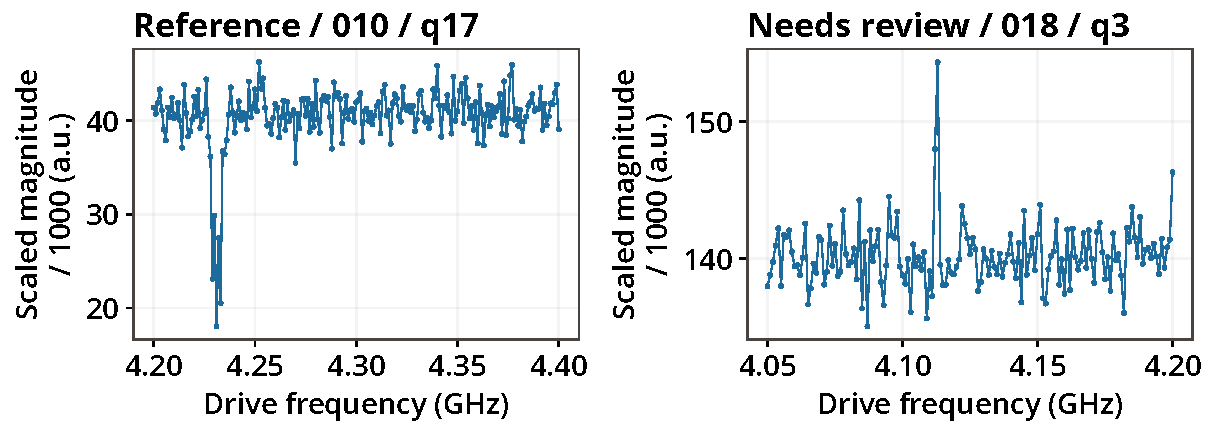
\includegraphics[width=\linewidth,height=34mm,keepaspectratio]{figures/spectroscopy-018.pdf}
\caption{左：对照 010；右：案例 018。IQ 投影诊断： $R^2=0.929$；步长 1.00 / 半高全宽 1.05 MHz。图示幅度；指标来自 IQ 投影的单洛伦兹线形拟合。}
\label{fig-spectroscopy-018}
\end{figure}
\endgroup
{\small\textbf{判断：线宽缺乏采样约束；需局部细扫并复测。}\par}
\end{frame}

\begin{frame}[t,label=case-readout-002]{两组准备条件的区分仍需验证}{GMM Readout Clusters / 002}
\setlength{\parskip}{0pt}
\begingroup
\setlength{\topsep}{0pt}\setlength{\partopsep}{0pt}
\begin{figure}
\centering
{\small
\makebox[.49\linewidth][c]{\textcolor{Teal}{左：准备条件较易区分}}%
\makebox[.49\linewidth][c]{\textcolor{Orange}{右：准备条件的分布仍有重叠}}\par
}
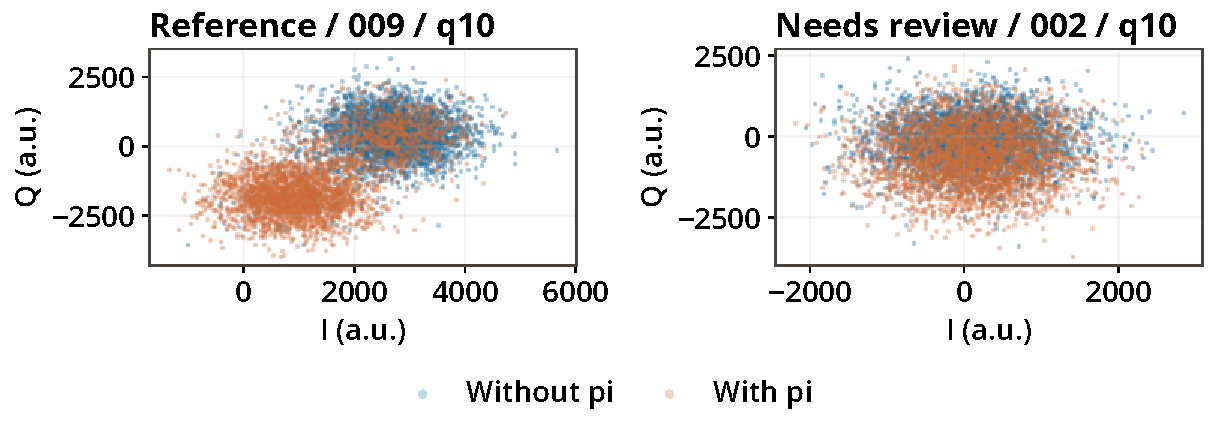
\includegraphics[width=\linewidth,height=34mm,keepaspectratio]{figures/readout-002.pdf}
\caption{左：对照 009；右：案例 002。线性分类器的留出评估平衡准确率： $62.12\%$。预测准备标签；包含状态准备与弛豫的影响。}
\label{fig-readout-002}
\end{figure}
\endgroup
{\small\textbf{判断：区分程度不足；需分别验证准备与读出，不能单独归因于测量。}\par}
\end{frame}

\begin{frame}[t,label=case-readout-003]{两组准备条件的区分仍需验证}{GMM Readout Clusters / 003}
\setlength{\parskip}{0pt}
\begingroup
\setlength{\topsep}{0pt}\setlength{\partopsep}{0pt}
\begin{figure}
\centering
{\small
\makebox[.49\linewidth][c]{\textcolor{Teal}{左：准备条件较易区分}}%
\makebox[.49\linewidth][c]{\textcolor{Orange}{右：准备条件的分布仍有重叠}}\par
}
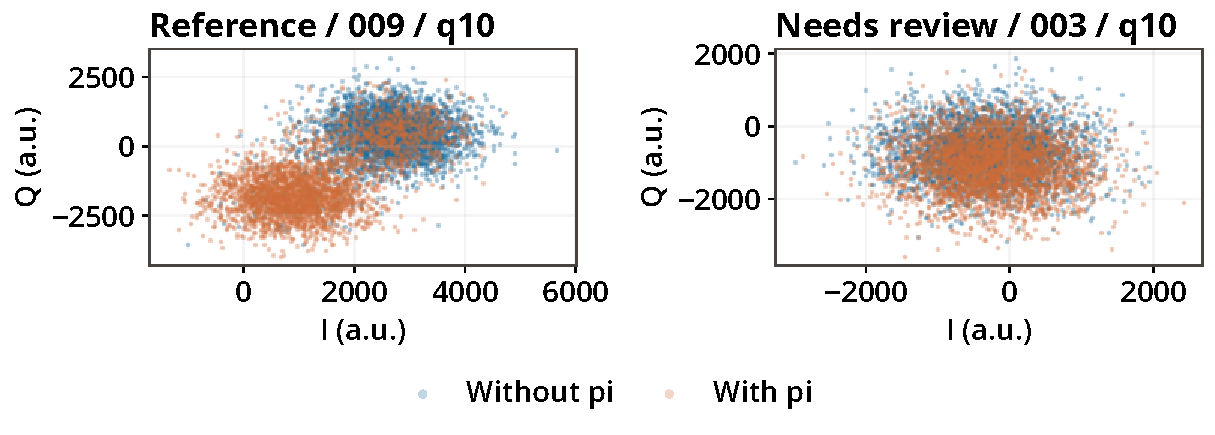
\includegraphics[width=\linewidth,height=34mm,keepaspectratio]{figures/readout-003.pdf}
\caption{左：对照 009；右：案例 003。线性分类器的留出评估平衡准确率： $59.67\%$。预测准备标签；包含状态准备与弛豫的影响。}
\label{fig-readout-003}
\end{figure}
\endgroup
{\small\textbf{判断：区分程度不足；需分别验证准备与读出，不能单独归因于测量。}\par}
\end{frame}

\begin{frame}[t,label=case-readout-004]{两组准备条件的区分仍需验证}{GMM Readout Clusters / 004}
\setlength{\parskip}{0pt}
\begingroup
\setlength{\topsep}{0pt}\setlength{\partopsep}{0pt}
\begin{figure}
\centering
{\small
\makebox[.49\linewidth][c]{\textcolor{Teal}{左：准备条件较易区分}}%
\makebox[.49\linewidth][c]{\textcolor{Orange}{右：准备条件的分布仍有重叠}}\par
}
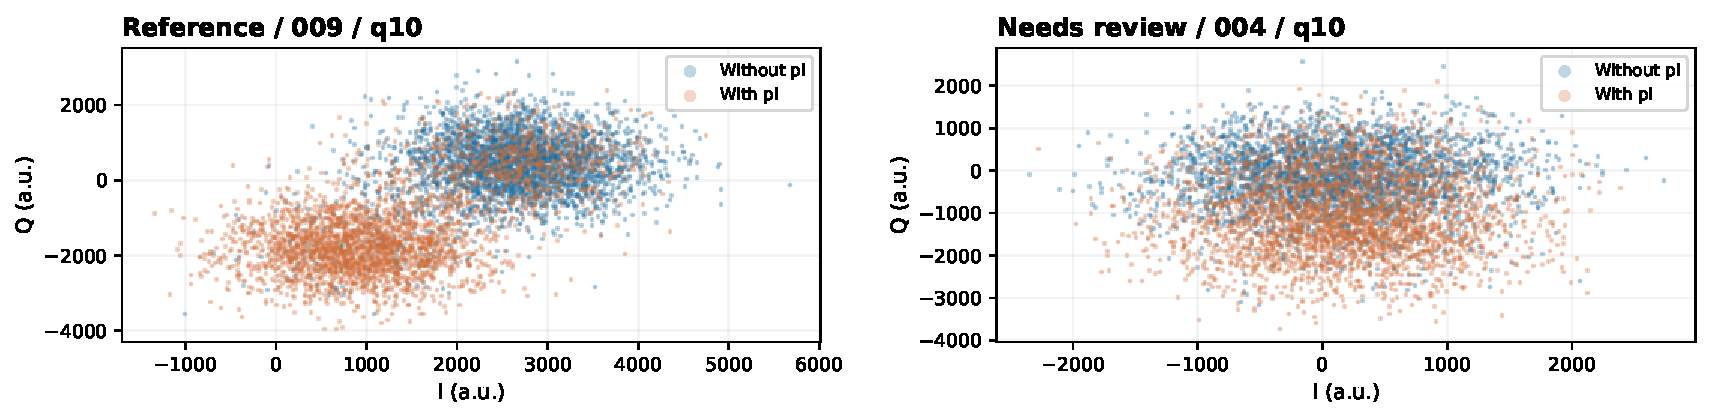
\includegraphics[width=\linewidth,height=34mm,keepaspectratio]{figures/readout-004.pdf}
\caption{左：对照 009；右：案例 004。线性分类器的留出评估平衡准确率： $70.73\%$。预测准备标签；包含状态准备与弛豫的影响。}
\label{fig-readout-004}
\end{figure}
\endgroup
{\small\textbf{判断：区分程度不足；需分别验证准备与读出，不能单独归因于测量。}\par}
\end{frame}

\begin{frame}[t,label=case-readout-005]{接近筛查阈值仍需结合数据判断}{GMM Readout Clusters / 005}
\setlength{\parskip}{0pt}
\begingroup
\setlength{\topsep}{0pt}\setlength{\partopsep}{0pt}
\begin{figure}
\centering
{\small
\makebox[.49\linewidth][c]{\textcolor{Teal}{左：准备条件较易区分}}%
\makebox[.49\linewidth][c]{\textcolor{Orange}{右：准确率略低于本地筛查阈值}}\par
}
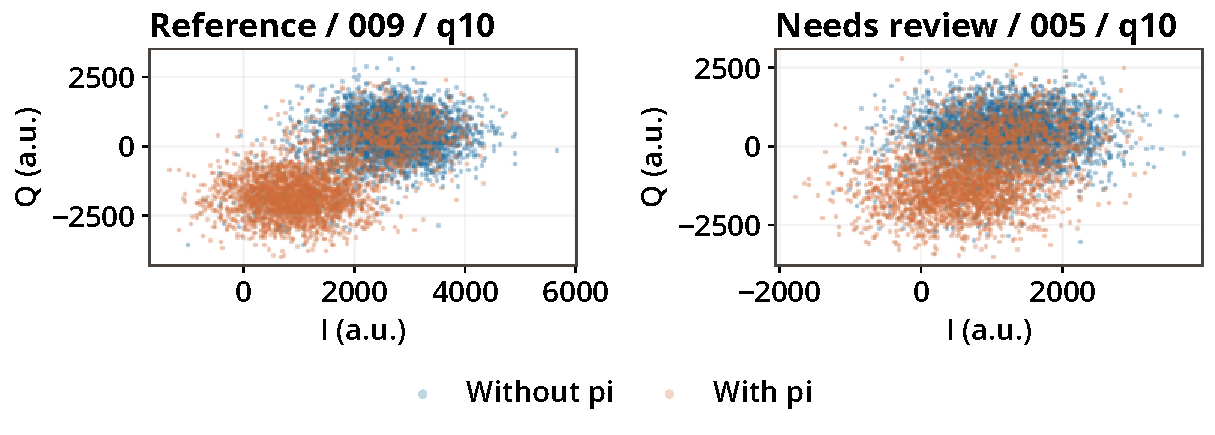
\includegraphics[width=\linewidth,height=34mm,keepaspectratio]{figures/readout-005.pdf}
\caption{左：对照 009；右：案例 005。线性分类器的留出评估平衡准确率： $74.48\%$。预测准备标签；包含状态准备与弛豫的影响。}
\label{fig-readout-005}
\end{figure}
\endgroup
{\small\textbf{判断：需结合重复测量判断；筛查阈值本身不构成物理失败标准。}\par}
\end{frame}

\fi
\end{document}
